\chapter{Experiments and Results}\label{results}

This chapter summarizes the experiments performed with the proposed model described in chapter \ref{approach}. In total, seven experiments were performed using the corpora outlined in the previous chapter. Along with the experiments, the results are also presented and compared with that of obtained using $\theta$RARes model wherever required. 

\section{Experiment-1: Performance on Small Corpus}

In order to see the performance of Word2Vec-$\theta$RARes model and Word2Vec-ESN classifier with the small corpus on the TRA task, the models were first tested with a limited number of sentences i.e. 26 sentences (sentence 15 to 40) from corpus-45. The chosen sentences have the distinct surface form and grammatical structure (e.g. active, passive, dative-passive). Using five instances of both the models, each model was first trained and tested on all the sentences to get the training errors and then tested using Leave one Out (LoO) cross-validation method: training on 25 sentences and testing on remaining one sentence such that all the sentences are tested at least once. Reservoir parameters for this experiments were optimized on 26 constructions used in the experiment by exploring the parameter space and using LoO cross-validation approach. This experiment remains a toy demonstration, and the generalization capability of the model will be investigated later with an extended corpus in Experiment-2 and Experiment-5.

\begin{table}[htbp]
\centering
\begin{threeparttable}
\caption[Cross-Validation errors with Word2Vec-$\theta$RARes on limited number of sentences.]{Generalization errors in SCL mode on 26 sentences of corpus-45.}
\label{tab:corpus_45_errors}
\rowcolors{2}{gray!25}{white}
\begin{tabular}{llcc}
\toprule
                           &              &  Word2Vec-$\theta$RARes     & $\theta$RARes \\
\midrule                 
\textbf{Meaning Error}    & mean         & 35.09                      & 14.83  \\
                        & std.         & 05.89                     & 02.59  \\
\textbf{Sentence Error}    & mean         & 85.38                      & 42.73 \\
                        & std.         & 07.88                     & 07.19 \\
\bottomrule
\end{tabular}
\begin{tablenotes}
\small
\item 
LoO cross-validation errors with both Word2Vec-$\theta$RARes model and $\theta$RARes model (shown in \%). Mean and std. is the average and standard deviation of errors over several model instances.
\end{tablenotes}
\end{threeparttable}
\end{table}

\paragraph{Word2Vec-$\theta$RARes Model:} For simulation with Word2Vec-$\theta$RARes model in this experiment, the model was operated in the SCL mode. Also, the reservoir of 1000 neurons and parameters $SR = 2.1$, $IS = 6.6$, $LR = 0.5$ were used. When trained and tested on all the 26 sentences, the model learned the sentences without any errors. However, during the cross-validation the model failed to generalize and yielded high cross-validation error rates (ME = $35.09\%$ and SE = $85.38\%$). This indicates that the Word2Vec-$\theta$RARes model is overfitting on the dataset. However, this is not surprising because the dataset contains limited examples, which constrained the model to generalize well. 

As illustrated in Table \ref{tab:corpus_45_errors}, it can be seen that the cross-validation errors with Word2Vec-$\theta$RARes model are almost doubled when compared to $\theta$RARes model. It is also important to know that the cross-validation errors of $\theta$RARes model reported in the Table \ref{tab:corpus_45_errors} are averaged over 100 reservoir instances of 100 units each \cite{xavier:2013:RT}. Whereas, the cross-validation errors of Word2Vec-$\theta$RARes are averaged over five reservoir instances of 1000 neurons each. With the small reservoir of 100 neurons, the Word2Vec-$\theta$RARes failed to learn and generalize (not reported here) on the same 26 sentences used in this experiment. This shows that the $\theta$RARes model performs better than the proposed Word2Vec-$\theta$RARes model on the small dataset even with a small reservoir.

\paragraph{Word2Vec-ESN classifier:} For simulation with Word2Vec-ESN classifier, a reservoir of size 500 neurons and parameters $SR = 0.2 $ , $IS = 0.7$ , $ LR = 0.7$, were used. As illustrated in Table \ref{tab:corpus_45_scores}, the Word2Vec-ESN classifier learned the 26 sentences resulting in F1-Score of $95.68\%$ during the training. While testing the classifier using LoO cross-validation method it generalized with low F1-Score of $68.53\%$. The high difference in F1-Score during training and testing conditions points toward the limited generalization capability of the classifier on unseen sentences. 

\begin{table}[htbp]
\centering
\begin{threeparttable}
\caption[Generalization score with Word2Vec-ESN classifier on limited number of sentences.]{Classification score of model Word2Vec-ESN classifier on 26 sentences from corpus-45.}
\label{tab:corpus_45_scores}
\rowcolors{2}{gray!25}{white}
\begin{tabular}{llccc}
\toprule
                   &              &  Precision         & Recall    & F1-Score\\
\midrule                
\textbf{training error}    & mean         & 94.92              & 96.54     & 95.68  \\
                & std.         & 00.27             & 00.74      & 00.46  \\
\textbf{test error}    & mean         & 69.87              & 71.29      & 68.53 \\
                & std.         & 02.36             & 01.37     & 01.80  \\
\bottomrule
\end{tabular}
\begin{tablenotes}
\small
\item 
LoO classification scores of Word2Vec-ESN classifier (shown in \%). Mean and std. is average and standard deviation of classification scores over several model instances.
\end{tablenotes}
\end{threeparttable}
\end{table}


\section{Experiment-2: Generalization Capabilities} \label{exp-2}

In the previous experiment, we saw the performance of both the proposed models with a limited number of sentences. The results indicated that the model is probably overfitting and not generalizing on the unseen sentences. Therefore, in this experiment, an extended corpus of 462 sentences (see section \ref{corpora}) was used to test the generalization capability of the models. The simulations were performed with five instances of both the proposed models each with a reservoir of 1000 neurons. To test the learning ability, both the models were initially trained and tested on all the sentences of the corpus-462. Also, to test the generalization ability of both the models, 10-fold cross-validation was used.  

\paragraph{Word2Vec-$\theta$RARes model:} 

In order to compare the learnability and generalization capability of the Word2Vec-$\theta$RARes and $\theta$RARes model, simulations were performed in both the SCL and SFL mode. Also, the reservoir parameters identified during grid search for both the learning modes were used i.e. $SR = 2.4$, $IS = 2.5$, $LR = 0.07$ in SCL mode and $SR = 2.2$, $IS = 2.3$ , $LR = 0.13$ SFL mode (see section \ref{grid_search} in chaper \ref{experiments}). 

%NOTE: 08/09/2016 results are copied after the simulation and are final, no need to change.
\begin{table}[htbp]
\centering
\begin{threeparttable}
\caption{Meaning and Sentence error in the SCL and SFL modes.}
\label{tab:corpus-462_errors}
\rowcolors{2}{white}{gray!25}
\begin{tabular}{llrrrrrrrr}
  \toprule
  \hiderowcolors   
  &  & \multicolumn{4}{c}{Word2Vec-$\theta$RARes} & \multicolumn{4}{c}{$\theta$RARes} \\
  \cmidrule(lr){3-6}   \cmidrule(lr){7-10}
  
  &  & \multicolumn{2}{c}{corpus-462} & \multicolumn{2}{c}{462 scrambled} & \multicolumn{2}{c}{corpus-462} & \multicolumn{2}{c}{462 scrambled} \\
  \cmidrule(lr){3-4} \cmidrule(lr){5-6}  \cmidrule(lr){7-8} \cmidrule(lr){9-10}  
  
  
                           &         & ME     & SE         & ME      & SE         & ME     & SE        & ME     & SE         \\
  \midrule
  \showrowcolors
  \textbf{SCL\ train}     & mean     & 0.55 & 1.64          & 6.68  & 26.80         & 0.12 & 1.21     & 4.81  & 20.43    \\
                           & std     & 0.06 & 0.12         & 0.67  & 1.64         & 0.03 & 0.30     & 0.30  & 1.25    \\
                           
  \textbf{SCL\ test}     & mean  & 8.68 & 24.09         & 70.15 & 99.26     & 7.43 & 32.13     & 74.15 & 99.89    \\
                             & std      & 1.01 & 2.38         & 1.24  & 0.29      & 0.52 & 1.35     & 0.80  & 0.15    \\
                             
  \textbf{SFL\ train}     & mean     & 0.16 & 0.52         & 9.38  & 35.58     & 0.00 & 0.00     & 0.00  & 0.00    \\
                           & std     & 0.09 & 0.25         & 0.69  & 3.40         & 0.00 & 0.00     & 0.00  & 0.00    \\
                           
  \textbf{SFL\ test}    & mean  & 8.88 & 25.17         & 67.87 & 99.26     & 9.18 & 24.37     & 73.39 & 99.91    \\
                            & std     & 0.14 & 0.01        & 0.10  & 0.33      & 0.57 & 1.19     & 0.96  & 0.11    \\
  \bottomrule
\end{tabular}
\begin{tablenotes}
\small
\item 
Meaning (ME) and Sentence error (SE) in different learning modes with Word2Vec-$\theta$RARes and $\theta$RARes model \cite{xavier:2013:RT}. The errors are given in percentage upto two decimal precision. SCL: Sentence Continuous Learning; SFL: Sentence Final Learning; std: standard deviations. Simulations were done with 5 model instances each with a reservoir of 1000 neurons.
\end{tablenotes}
\end{threeparttable}
\end{table}

Table \ref{tab:corpus-462_errors} illustrates the train and test errors obtained with Word2Vec-$\theta$RARes and $\theta$RARes model. One can see that while training both the Word2Vec-$\theta$RARes and $\theta$RARes model learned all the sentences thoroughly (less than $ 1\% $ error rates) in both the SCL and  SFL mode. Comparing the performance during testing, we can see an improvement of $8.04 \%$ sentence error in SCL mode with Word2Vec-$\theta$RARes model, whereas the meaning error dropped by $1.25 \%$. However, considering the standard deviation, we can also say that the meaning error remained almost equivalent in both the Word2Vec-$\theta$RARes and $\theta$RARes model. In SFL mode, both the meaning and sentence errors remained nearly equal for both the models. It can also be observed that with Word2Vec-$\theta$RARes model performs better in SCL mode when compared to SFL mode, whereas it is vice-versa in $\theta$RARes model. Additionally, the Word2Vec-$\theta$RARes model outperform the $\theta$RARes model in SCL mode.

The same experiment was also performed using the sentence in corpus-462 without the topologically modified coded meaning. The cross-validation errors were found to be negligibly increased ($\approx 1 \%$ in SCL mode and $\approx 3 \%$ in SFL mode ) but with the different reservoir parameters (SR = 3.9, IS = 3.8, LR = 0.1 in SCL mode and SR=3.2, IS=3.9, LR=0.1 in SFL mode). This supports the suggestions of Hinaut et al. \cite{xavier:2013:RT}, that topologically modified coded meaning of a sentence (see fig. \ref{fig:w2v_esn_nv}) is equivalent to the usual coded meaning (see fig. \ref{fig:model_variant_1}). Even without the modified coded meaning the Word2Vec-$\theta$RARes model performed better than $\theta$RARes model in SCL mode.

\paragraph{Word2Vec-ESN classifier:} 

Recall that unlike Word2Vec-$\theta$RARes model, the performance of Word2Vec-ESN classifier is evaluated using classification metrics (see section \ref{sec:model_variant}). The classifier process the raw sentences and the distributed vector representation of the input argument-predicate pair is fed into ESN. In order to see the effect of distributed word vectors over localist word representation, it is also important to test the behavior of the classifier on the sentences transformed to grammatical form and using localist word representation as an input to ESN. Thus for this experiment, simulations were performed with the Word2Vec-ESN classifier in two configurations mentioned below.

\begin{enumerate}
\setlength{\itemsep}{\smallskipamount}

\item \textbf{Configuration-1: } In this configuration, the Word2Vec-ESN classifier process the raw sentences and distributed vector representation of the argument-predicate pairs are input to ESN (see section \ref{sec:model_variant} for more detail). For the simulation in this configuration, the reservoir parameters $SR = 0.7$ , $IS = 1.15$, $LR = 0.1$ were used. The parameters are identified previously by exploring the parameter space. \label{config-1}

\item \textbf{Configuration-2: } In this configuration, the Word2Vec-ESN classifier was used without the Word2Vec unit, and only the ESN is used for processing the sentences. The input sentences were transformed in the grammatical form: all the semantic words in the sentence were replaced with `SW' token, and the localist word vectors are input to ESN. For the simulation in this configuration, the reservoir parameters $SR = 1.3$, $IS = 1.0$ , $LR = 0.4$ found previously during grid search were used. \label{config-2}

\end{enumerate} 

\begin{table}
\centering
\begin{threeparttable}
\caption{Classification scores of the Word2Vec-ESN classifier on unscrambled and scrambled corpus-462 in two configurations.}
\label{tab:corpus-462-scores}
\rowcolors{2}{white}{gray!25}
\begin{tabular}{llllll}
  \toprule
  \hiderowcolors   
  &  & \multicolumn{2}{c}{Configuration-1} & \multicolumn{2}{c}{Configuration-2} \\
  \cmidrule(lr){3-4}    \cmidrule(lr){5-6} 
  &  & \multicolumn{1}{c}{corpus-462} & \multicolumn{1}{c}{462 scrambled} & \multicolumn{1}{c}{corpus-462} & \multicolumn{1}{c}{462 scrambled} \\
               
  \midrule
  \showrowcolors
  \textbf{Precision}     & test         & 96.76 ($\pm$ 0.08) & 95.72 ($\pm$ 0.15)    & 61.91 ($\pm$ 0.07) & 16.71 ($\pm$ 0.64)     \\
                             & train     & 97.46 ($\pm$ 0.00) & 96.96 ($\pm$ 0.13)    & 61.96 ($\pm$ 0.07) & 57.24 ($\pm$ 7.90)    \\
                           
  \textbf{Recall}         & test      & 91.78 ($\pm$ 0.08) & 89.75 ($\pm$ 0.11)    & 68.20 ($\pm$ 0.46) & 20.01 ($\pm$ 0.02)     \\
                             & train     & 92.29 ($\pm$ 0.22) & 90.40 ($\pm$ 0.05)    & 67.69 ($\pm$ 0.29) & 20.17 ($\pm$ 0.04)    \\
                             
  \textbf{F1-Score}     & test         & 93.99 ($\pm$ 0.09) & 92.28 ($\pm$ 0.12)     & 63.71 ($\pm$ 0.22) & 17.49 ($\pm$ 0.05)    \\
                           & train     & 94.65 ($\pm$ 0.00) & 93.24 ($\pm$ 0.08)    & 63.55 ($\pm$ 0.17) & 17.74 ($\pm$ 0.08)    \\                           
  
  \bottomrule
\end{tabular}
\begin{tablenotes}
\small
\item 
{\small Classification scores (in  $\%$) of Word2Vec-ESN classifier during training and testing conditions. Configuration-1: raw sentences are processed, and distributed vectors of the argument-predicate pairs are input to ESN. Configuration-2: Sentences transformed to grammatical form and localist word vectors are input to ESN. Simulations were performed with five instances of Word2Vec-ESN classifier each with a reservoir of 1000 neurons.}
\end{tablenotes}
\end{threeparttable}
\end{table}

Table \ref{tab:corpus-462-scores} illustrates the training and cross-validation classification scores of simulations performed with the Word2Vec-ESN classifier in both the configurations. The classifier in configuration-1 learned and generalized on the corpus with high classification scores whereas, in configuration-2, the classifier learned the corpus with low classification scores and hence failed to generalize as shown by low scores. Notice the marginal difference between the training and cross-validation scores in configuration-1. This indicates that the Word2Vec-ESN classifier is generalizing with high classification scores on the unseen sentences and do not overfit. Comparing the performance of the classifier in both the configurations, it can be observed that the classifier performed better when the distributed word embeddings were used as an input to ESN (i.e. configuration-1) as compared to the use of localist words vectors as an input to the ESN (i.e. configuration-2).

% CONFUSION MATRIX
\begin{figure}[hbtp]
\centering
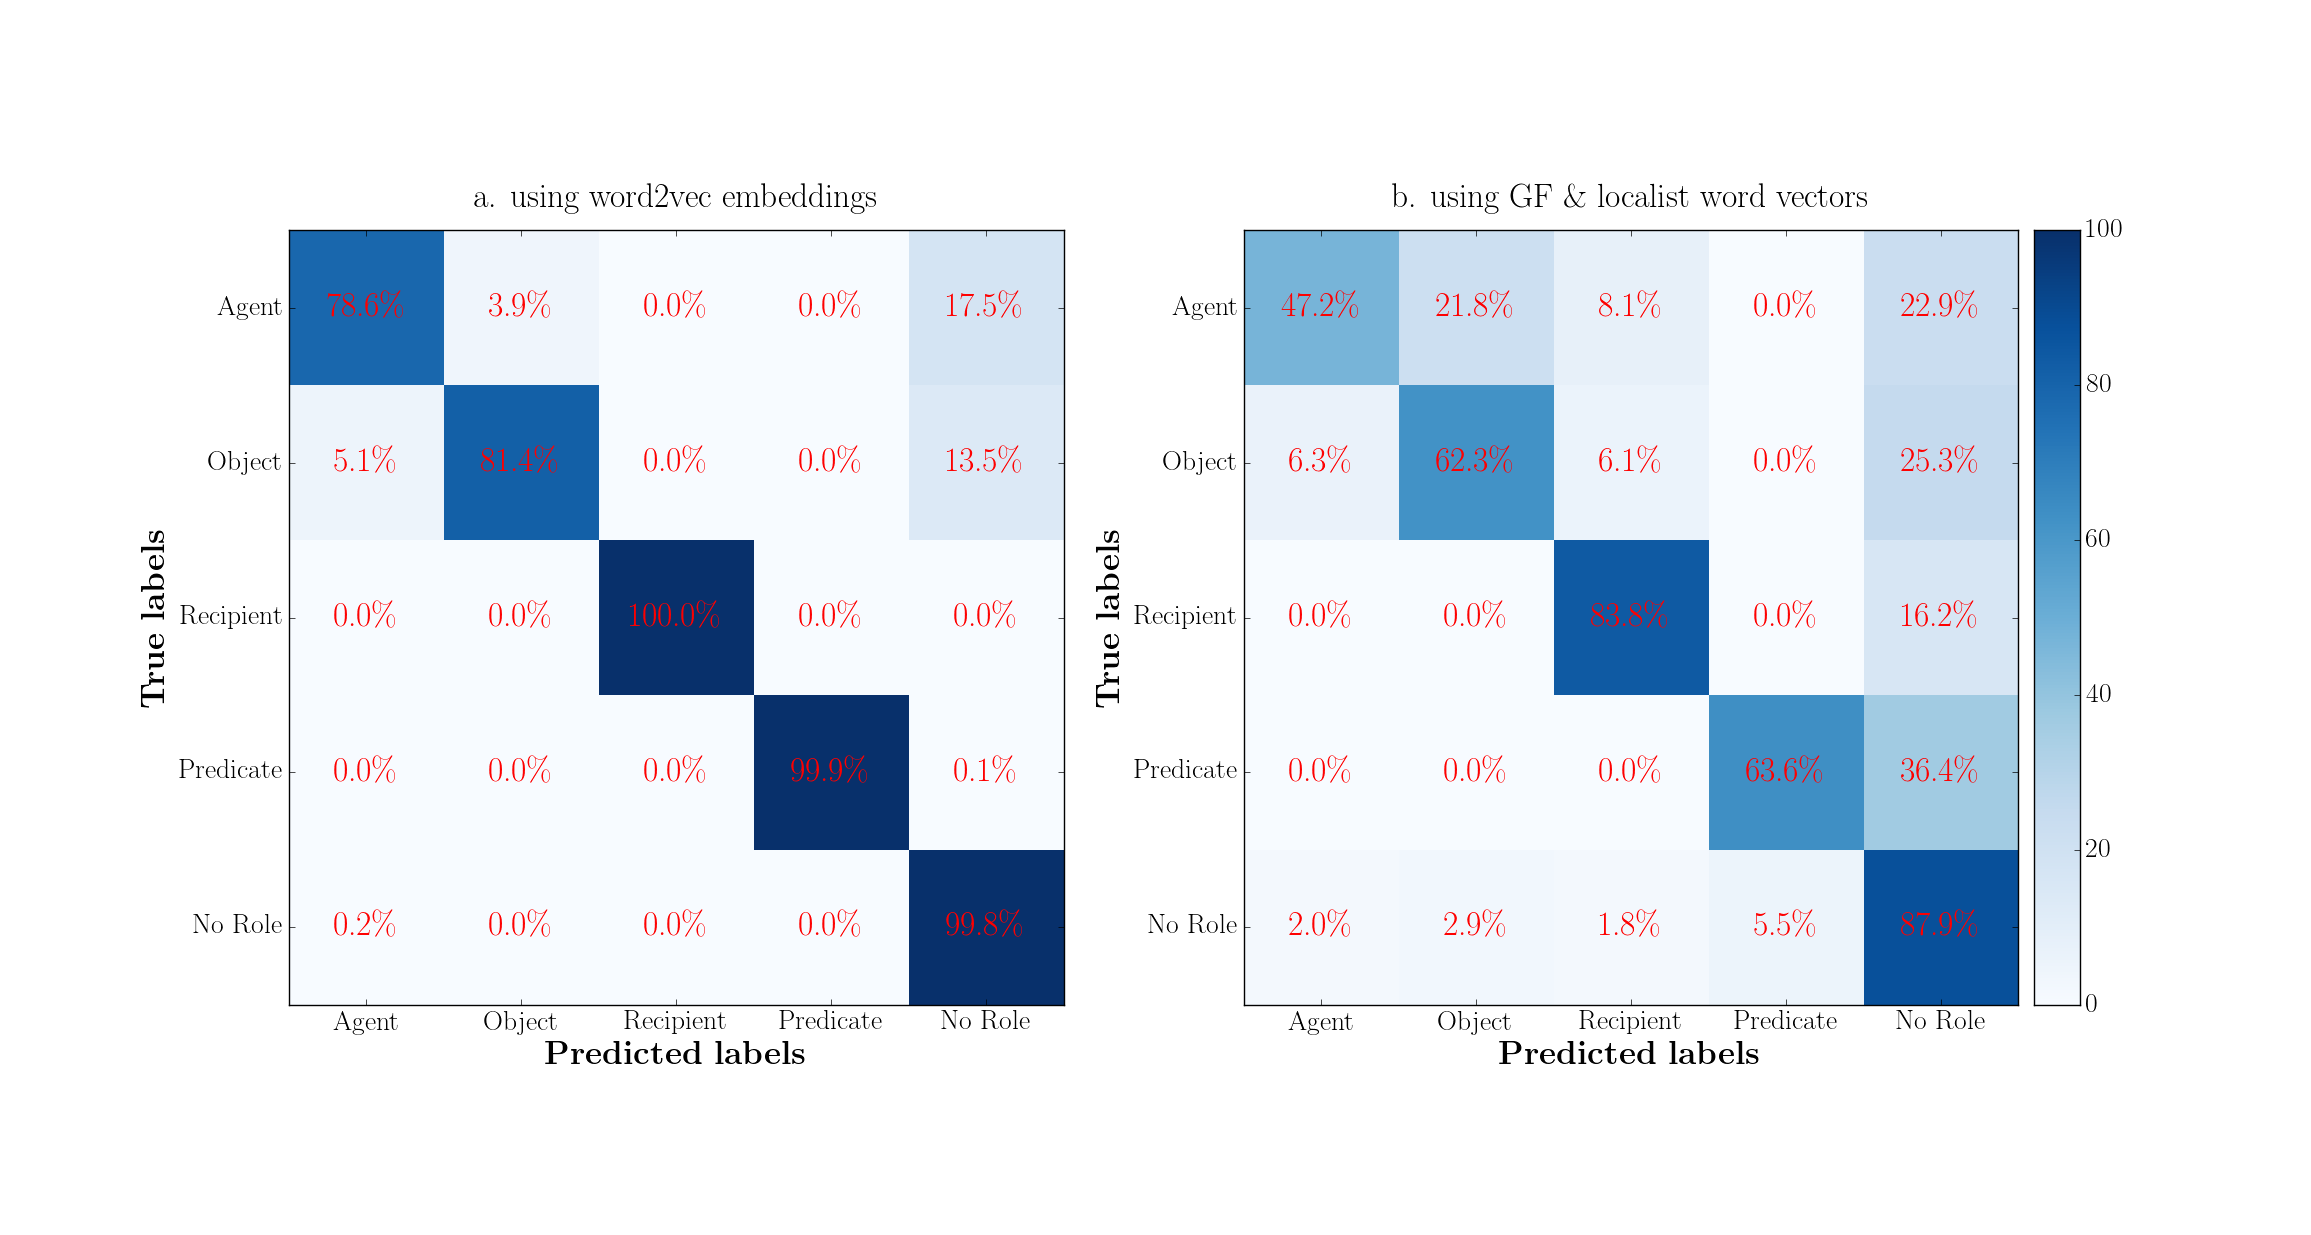
\includegraphics[width=1.0\linewidth]{confusion_matrix}
\caption[Normalized confusion matrix for unscrambled corpus-462.] {\textbf{Normalized confusion matrix with Word2Vec-ESN classifier in configuration-1 and configuration-2:}{\small The confusion matrix with true roles (in rows) and predicted roles (in columns). The top-left to bottom-right diagonal shows the percentage of words whose roles are predicted correctly. Everything other than this diagonal represents the incorrect prediction of roles. Configuration-1: raw sentences processed by Word2Vec-ESN classifier and word2vec word vectors are input to ESN. Configuration-2: Sentences transformed to grammatical form and localist word vectors are input to ESN. The results were obtained with reservoir of 1000 neurons and 10-fold cross-validation.}}
\label{fig:confusion_matrix}
\end{figure}

% CONFUSION MATRIX SCRAMBLED
\begin{figure}[hbtp]
\centering
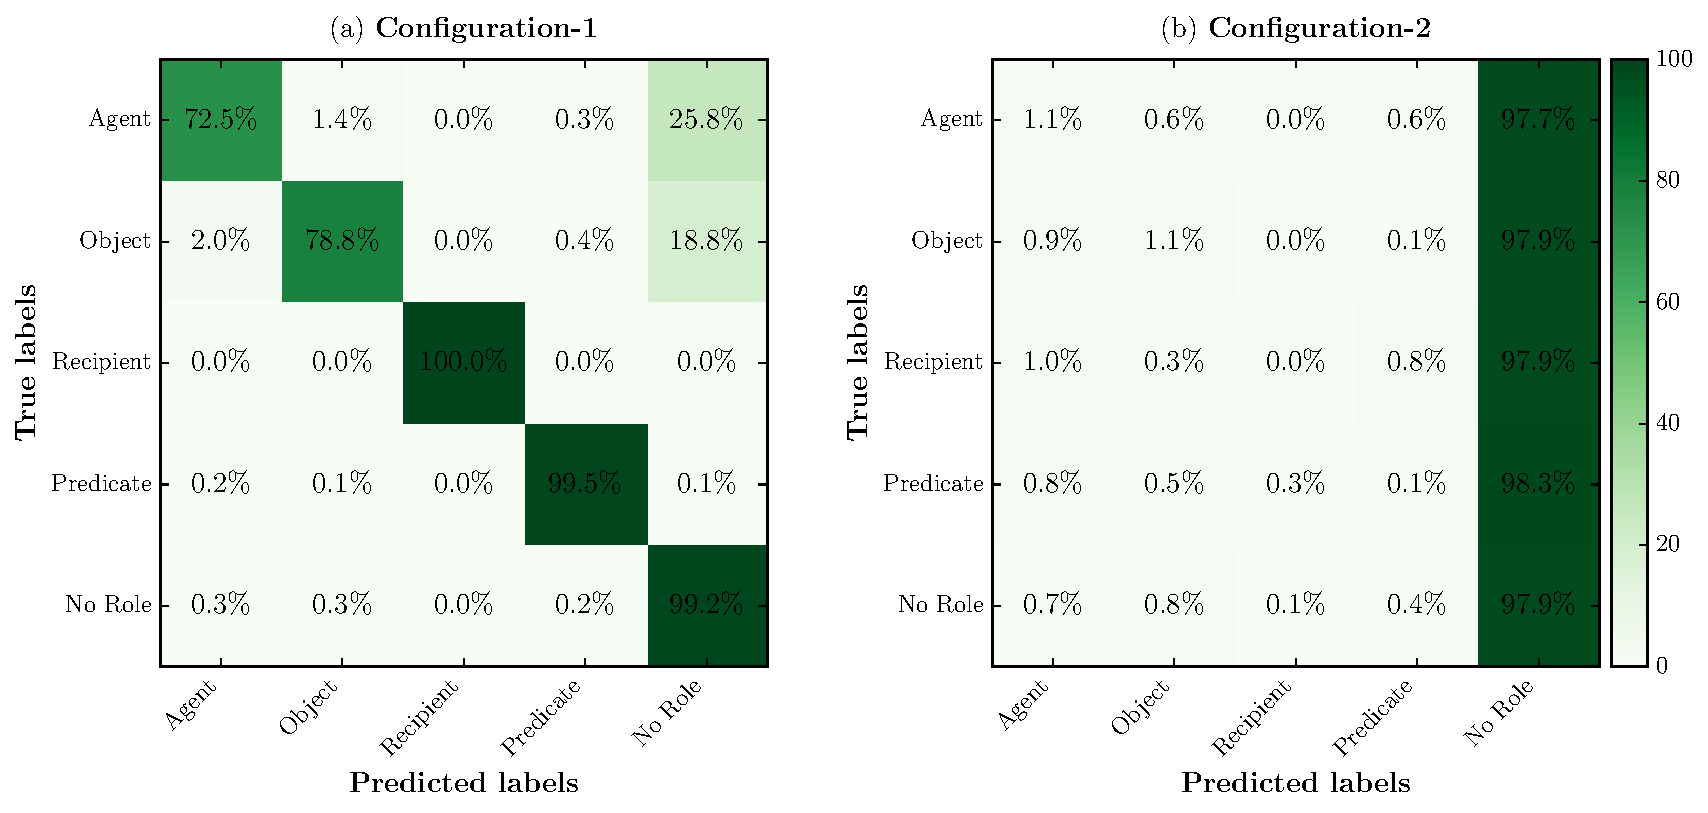
\includegraphics[width=1.0\linewidth]{confusion_matrix_shuffle}
\caption[Normalized confusion matrix for scrambled corpus-462.] {\textbf{Normalized confusion matrix with the Word2Vec-ESN classifier on scrambled corpus-462: } {\small The confusion matrix shows the true roles (in rows) and predicted roles (in columns) of argument-predicate pairs. The top-left to bottom-right diagonal shows the percentage of argument-predicate pairs for which the roles are predicted correctly. All cells, other than this diagonal represents the incorrect prediction of the roles. Configuration-1: raw sentences processed by the Word2Vec-ESN classifier and distributed word vectors are input to ESN. Configuration-2: Sentences transformed to grammatical form and localist word vectors are input to ESN. The results were obtained with reservoir of 1000 neurons.}}
\label{fig:confusion_matrix_shuffle}
\end{figure}

Figure \ref{fig:confusion_matrix} shows the confusion matrices of true and predicted roles for input argument-predicate pairs in confguration-1 and configuration-2. The matrices are plotted using the cross-validation results of the Word2Vec-ESN classifier. The corresponding classification scores of the individual roles produced by the classifier during 10-fold cross-validation are also reported in Table \ref{tab:classsification-scores-21} for both the configurations.

As shown in the confusion matrix (see fig. \ref{fig:confusion_matrix}), it can be observed that when using the distributed vectors of argument-predicate pair as an input to ESN (i.e. configuration-1), the model predicted the roles `Recipient', `Predicate' and `No Roles' almost without making any errors. Notice that the classifier mispredicted the roles `Agent' and `Object' mostly as `No Role'. It can also be noticed that the roles `Agent' and `Object' were confused with each other i.e. the argument-predicate pairs with the role `Agent' were misclassified as `Object' and vice-versa. 

Using the sentences in grammatical form along with the localist word vectors of the argument-predicate pairs (i.e. configuration-2), as an input to ESN, the roles `Recipient' and `No Role' were predicted correctly with least errors of $16.2 \%$ and $12.1 \%$. Notice that significant amount of all the roles were misclassified as `No Role', where the `Predicate' being the highest role to be misclassified ($36.4 \%$) as `No Role'. The classifier in configuration-2 also seems to be confused between the roles `Agent' and `Object'. Additionally, the argument-predicate pairs with the true roles `Agent' and `Object' were also confused with the role `Recipient'. 

While comparing the predictions made by the Word2Vec-ESN classifier in both the configurations, it was observed that the roles `Agent' and `Object' made the most number of errors in predictions as compared to other roles. In both the configurations, the model was mainly confused between roles `Agent' and `Object', but with the higher number of misclassification in configuration-2. Additionally, in configuration-2, the roles `Agent' and `Object' were wrongly predicted as `Recipient', whereas in configuration-1, this misprediction does not exist. Comparing the false predictions made by the classifier in both the configurations, it can be observed that the number of incorrect predictions was comparatively less in configuration-1. Also, in configuration-1, all the argument-predicate pairs with actual roles `Recipient', `Predicate' and `No Role' were predicted almost without any errors whereas, in configuration-2, the classifier misclassified these roles respectively by $16.2 \%$, $36.4\%$, and $12.1 \%$.


%NOTE: 08/09/2016 results are copied after the simulation and are final, no need to change.
\begin{table}[h]
\centering
\begin{threeparttable}
\caption{Training and testing classification scores for individual roles when using Word2Vec-ESN classifier in two different configurations.}
\label{tab:classsification-scores-21}
\rowcolors{2}{gray!25}{white}
\begin{tabularx}{\textwidth}{llYYYYYYY}
\hiderowcolors
\toprule
  &  & \multicolumn{3}{c}{Configuration-1} & \multicolumn{3}{c}{Configuration-2}& \\  
\cmidrule(lr){3-5}   \cmidrule(lr){6-8}
   
Role                 &             & Pr   & Re  & F1         & Pr  &  Re & F1         &  Support  \\
\showrowcolors
\midrule
               
\textbf{Agent}        &test         & 0.92 & 0.79 & 0.85     & 0.63 & 0.47 & 0.54    & 888  \\
                    &train      & 0.94 & 0.80 & 0.86     & 0.64 & 0.46 & 0.53    & 892  \\
\textbf{Object}        &test         & 0.95 & 0.81 & 0.88     & 0.51 & 0.62 & 0.56    & 791  \\
                    &train      & 0.96 & 0.82 & 0.88     & 0.51 & 0.61 & 0.56    & 794  \\
\textbf{Recipient}    &test         & 1.00 & 1.00 & 1.00     & 0.52 & 0.84 & 0.64    & 382  \\
                    &train      & 1.00 & 1.00 & 1.00     & 0.52 & 0.83 & 0.64    & 384  \\
\textbf{Predicate}    &test        & 1.00 & 1.00 & 1.00     & 0.51 & 0.64 & 0.57    & 888  \\
                    &train      & 1.00 & 1.00 & 1.00     & 0.51 & 0.64 & 0.57    & 892   \\
\textbf{No Role}    &test         & 0.97 & 1.00 & 0.99     & 0.92 & 0.88 & 0.90    & 9776  \\
                    &train      & 0.97 & 1.00 & 0.99     & 0.91 & 0.88 & 0.90    & 9823  \\
\bottomrule
\end{tabularx}
\begin{tablenotes}
\small
\item Training and cross-validation classification scores (precision upto 2 decimals) for each output roles predicted by the Word2Vec-ESN classifier in two configuration. Support for each role: actual number of instances, is also shown in last column. Simulation condition: 1000 reservoir neurons, 10-fold cross-validation.
\end{tablenotes}
\end{threeparttable}
\end{table}

\section{Experiment-3: Effect of Corpus Structure} 

As described earlier, the sentences in the corpus-462 were created based on context-free grammar. Thus the sentences in the corpus contain an inherent grammatical structure. The models are thus possibly utilizing the underlying grammatical structure to some extent for learning and generalization. To test this hypothesis and to demonstrate that the models are not generalizing on any other inconsistent regularity in the corpus, in this experiment, the inherent grammatical structure from the sentences of corpus-462 was removed by randomizing the word orders within the sentences \cite{xavier:2013:RT}. Such a test will also help us to have an insight on what the model is actually learning and whether the model is overfitting or not. 

For the simulations, the corpus-462 with the scrambled sentences (i.e. in the absence of any grammatical structure) was presented to the Word2Vec-$\theta$RARes model and Word2Vec-ESN classifier. Keeping all conditions and the reservoir parameters same as used in Experiment-2 for both the models, a 10-fold cross-validation was performed with five model instances. Apart from cross-validation, the models were also trained and tested on all the sentences in the corpus to determine the learning ability of the models with the scrambled corpus.

\paragraph{Word2Vec-$\theta$RARes model:}

As illustrated in Table \ref{tab:corpus-462_errors}, it was observed that when using the scrambled corpus as an input to the Word2Vec-$\theta$RARes model, the model learned the scrambled sentences with low error rates of $ME = 6.68 \%$ and $SE = 26.80 \%$ in SCL mode. While testing, the model generalized with cross-validation error rates of $ME = 70.15 \% $ and $SE = 99.26 \%$. Similarly, in SFL mode the model learned with low error rates of $ME = 9.38 \%$ and $SE = 35.58 \%$  but during cross-validation high error rates of $ME = 67.87 \%$ and $SE = 99.26 \% $ was observed. Notice that the model learned the scrambled corpus with low error rates while training, but during the cross-validation, it generalized with high error rates. While comparing the results of Word2Vec-$\theta$RARes model with and without inherent grammatical structures in the sentences, it can be observed that the model did not perform better on the corpus with the scrambled sentences. This indicates that the model is not generalizing on any other inconsistent regularity in the corpus, but instead utilizing the grammatical structure present in the sentences.


\paragraph{Word2Vec-ESN classifier:} Table \ref{tab:corpus-462-scores} illustrates the effect of the scrambled corpus on the Word2Vec-ESN classifier. It can be observed that in the configuration-1, the classification scores in training and testing conditions, remained almost equivalent to the scores obtained with the unscrambled corpus. Whereas in configuration-2, the Word2Vec-ESN classifier learned and generalized on the scrambled corpus with low classification scores. Also in configuration-2, notice the classification scores in both the training and testing conditions are lower than that obtained with the unscrambled corpus. 

Figure \ref{fig:confusion_matrix_shuffle} shows the confusion matrix obtained when the scrambled corpus is exposed to Word2Vec-ESN classifier. It was observed that in configuration-1, the Word2Vec-ESN classifier classifies the argument-predicate pair to the respective roles with high classification scores whereas, in configuration-2, it fails to do so. Comparing the confusion matrix obtained when using unscrambled corpus-462 (see fig. \ref{fig:confusion_matrix}) and scrambled corpus-462 (see fig. \ref{fig:confusion_matrix_shuffle}) it is clearly visible that in configuration-1, the classification scores for each role is negligibly affected whereas in configuration-2, the classification scores of individual roles dropped heavily.

\section{Experiment-4: Effect of Reservoir Size}

The most important hyperparameter which affects the performance of the proposed models is the size of the reservoir (i.e. $N_{x}$ = number of neurons in the reservoir). The addition of neurons in the reservoir is computationally inexpensive because the read-out weights ($W^{out}$) scales linearly with the number of neurons in the reservoir \cite{esn:learn_gs}. Liu et al. \cite{overfitting:liu} argued that as the number of neurons in the neural network increases, so does the danger of overfitting, thus ensuring the failure of the network to generalize during cross-validation. So, in order to determine the effect of reservoir size on the performance of the Word2Vec-$\theta$RARes model and Word2Vec-ESN classifier, the simulations were performed over a range of reservoir sizes \footnote[1]{Reservoir sizes explored in Word2Vec-$\theta$RARes model: [90, 291, 493, 695, 896, 1098, 1776, 2882, 3988, 5094]} \footnote[2]{Reservoir sizes explored in Word2Vec-ESN classifier: [50, 100, 250, 400, 600, 800, 1050, 1600, 2250, 3320, 3860, 4500]} with the five instances of the proposed models. The sizes of the reservoir were randomly chosen from a range of 50 to 5500 neurons. Also, for the simulations, corpus-462 was used, and models were tested using 10-fold cross-validation approach.

\paragraph{Word2Vec-$\theta$RARes model: } 

With the Word2Vec-$\theta$RARes model, simulations were performed on a range of reservoir size\footnotemark[1] in both the SCL and SFL modes, using the same optimal reservoir parameters as used in Experiment-2 i.e. $SR = 2.4$, $IS = 2.5$ and $LR = 0.07$ in SCL mode and $SR = 2.2$, $IS = 2.3$ and $LR = 0.13$ in SFL mode. 

\begin{figure}[hbtp]
\centering
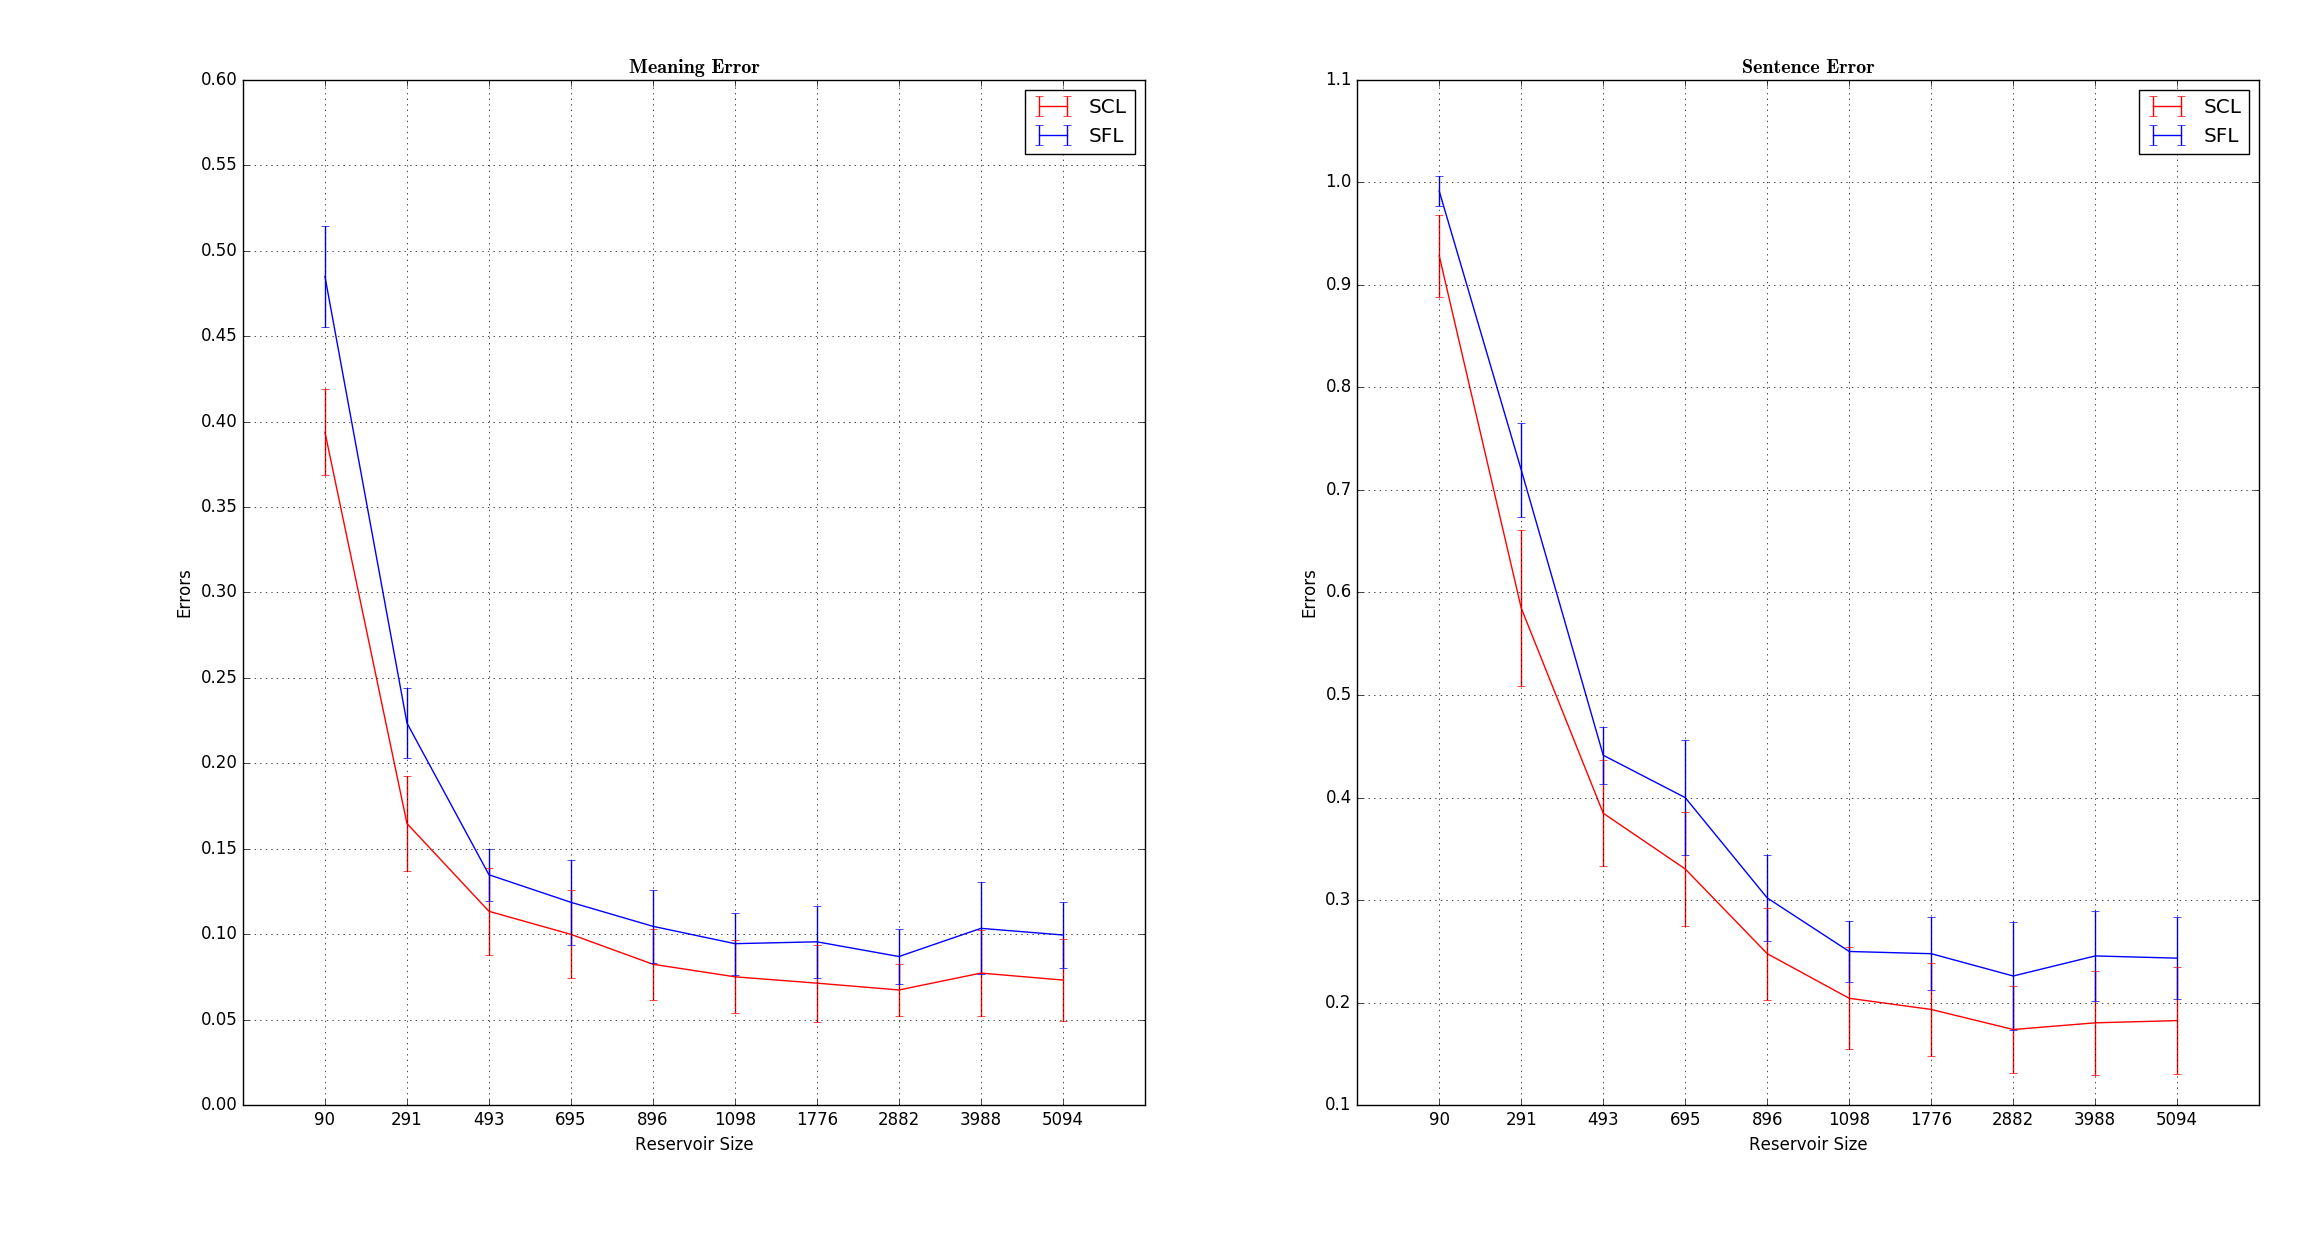
\includegraphics[width=1.0\linewidth]{reservoir_size_1}
\caption[Effect of reservoir size on Word2Vec-$\theta$RARes model.]{Effect of reservoir size on cross-validation errors of Word2Vec-$\theta$RARes model. NOTE: the scale of cross-validation error for the meaning and sentence error are different.}
\label{fig:reservoir_size_1}
\end{figure}

Figure \ref{fig:reservoir_size_1} shows the effect of reservoir size on the cross-validation errors rates (i.e. meaning and sentence error). The meaning and sentence errors continuously drop with the increase in reservoir size from 90 to 1098 in both the learning modes.  As the reservoir size is further increased from 1098, the meaning and sentence error in both the SCL and SFL mode is negligibly affected. Notice that with the increase in reservoir size, the meaning and sentence error curves follows the similar trend in both the SCL and SFL mode. Another interesting pattern to notice is that, with all the reservoir sizes studied, the meaning and sentence error in SCL mode is always lower than in SFL mode. Overall the important behavior to notice is that both the meaning and sentence cross-validation error rates reduce with the increase in the reservoir size, but asymptotes when the reservoir size is above 1000 neurons.

\paragraph{Word2Vec-ESN classifier: } 

To determine the effect of reservoir size on the Word2Vec-ESN classifier, simulations were performed on a range of reservoir sizes \footnotemark[2], in configuration-1 and configuration-2 of the classifier as described in Experiment-2. Also, for the simulations, reservoir parameters were kept identical to that used in Experiment-2.

\begin{figure}[hbtp]
\centering
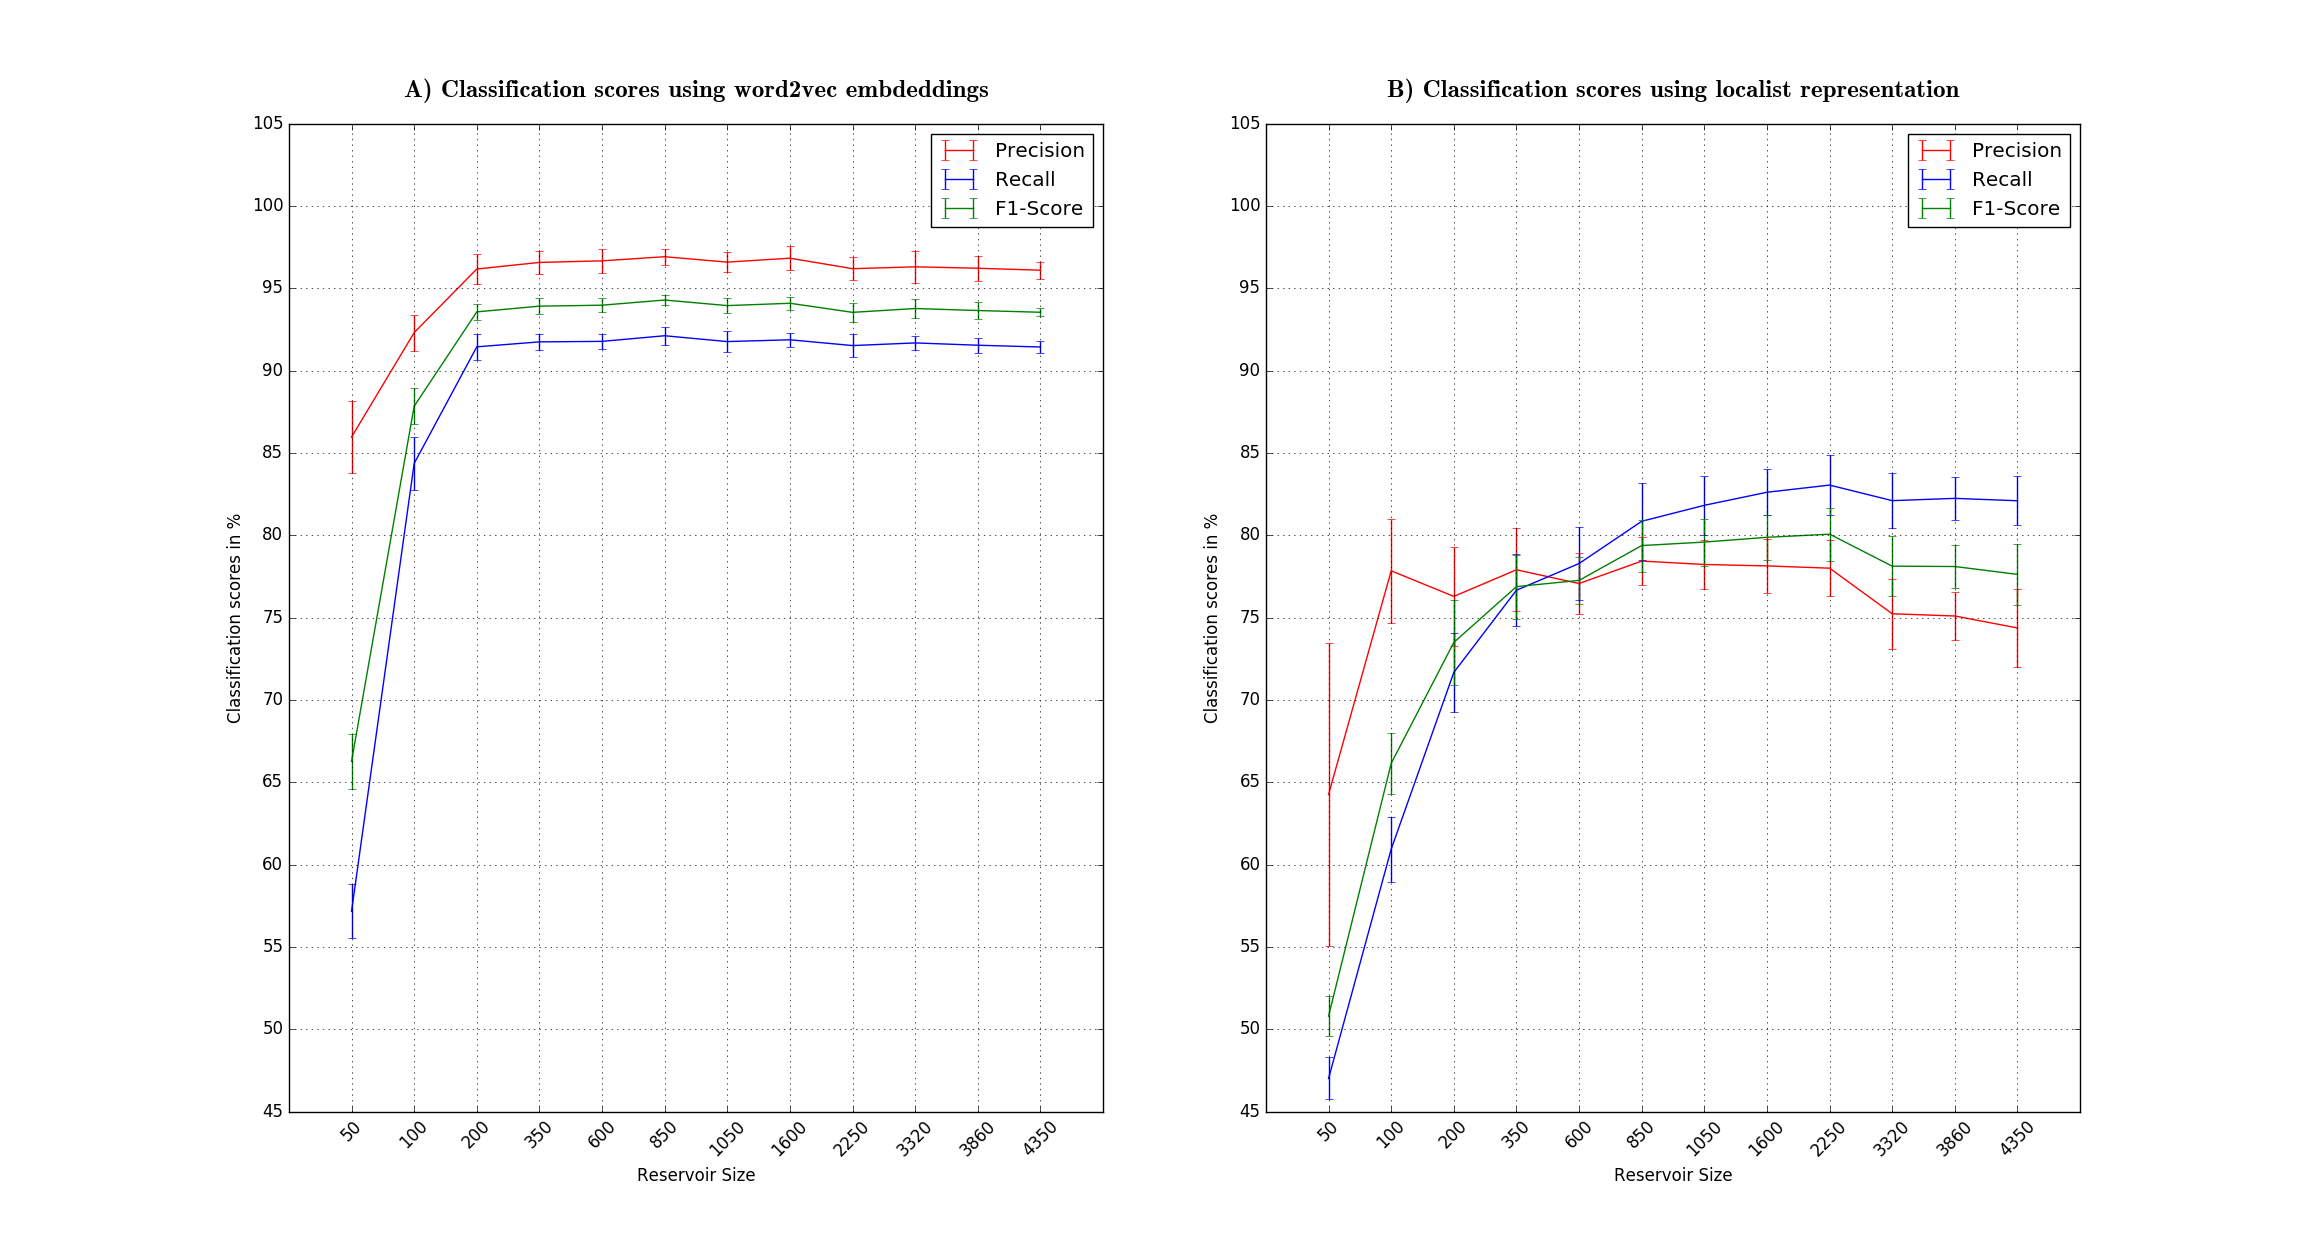
\includegraphics[width=1.0\linewidth]{reservoir_size_2}
\caption[Effect of reservoir size on Word2Vec-ESN classifier.]{Effect of reservoir size on classification scores of Word2Vec-ESN classifier. NOTE: the scale of cross-validation scores in configuration-1 and configuration-2 are different.}
\label{fig:reservoir_size_2}
\end{figure}

Figure \ref{fig:reservoir_size_2} shows the change in classification scores of the Word2Vec-ESN classifier with the increase in reservoir size. It can be observed that when using the distributed word vectors (i.e. configuration-1) the classification scores sharply increases when the reservoir size is increased from 50 neurons to 250 neurons. As the reservoir size is further increased from 250 neurons, the classification scores remain stable with the negligible drop of scores. Whereas in configuration-2 i.e. when using the sentences in grammatical form encoded using localist representation, the classification scores also improve, with the increase in reservoir size from 50 to 250 neurons. As the reservoir size is further increased from 250 neurons, the recall score is improved whereas the precision remains almost flat with negligible improvement. The F1-Score is harmonic mean of precision and recall, and thus it is also slightly increased. Notice that even the highest F1-Score of Word2Vec-ESN classifier observed at reservoir size 4500 in configuration-2 is much lower than that of observed at reservoir size 100 ($\approx 29 \%$ ) in configuration-1.

\section{Experiment-5: Scalability of the Model}

In order to investigate the effect of corpus size and to determine the scaling capability of the model, the extended corpus-90582 (see section \ref{corpora}) was used for this experiment. As this corpus also contains $12\%$ of ambiguous sentences \cite{xavier:2013:RT} which impede the learning and generalization of the model, this experiment will also validate the model's ability to process the ambiguous sentences. Thus, in order to study the scaling capability of the model with different corpus size, 6 sub-corpora were created by randomly sampling $6\%$, $12\%$, $25\%$, $50\%$, $75\%$, $100\%$ of sentences from the original corpus of 90582 sentences \cite{xavier:2013:RT}. Each of the generated sub-corpora was exposed to the Word2Vec-$\theta$RARes model, and a 2-fold cross-validation was performed. The model was trained on half the sub-corpora size and tested on remaining half. The second half used for testing was then used to train the model and tested on the first half, used for training previously. This experiment was performed with the Word2Vec-$\theta$RARes model in both learning modes i.e. SCL and SFL, using five model instances each with a reservoir of 5000 neurons. All the other reservoir parameters were kept identical to the Experiment-2.

\begin{figure}[hbtp]
\centering
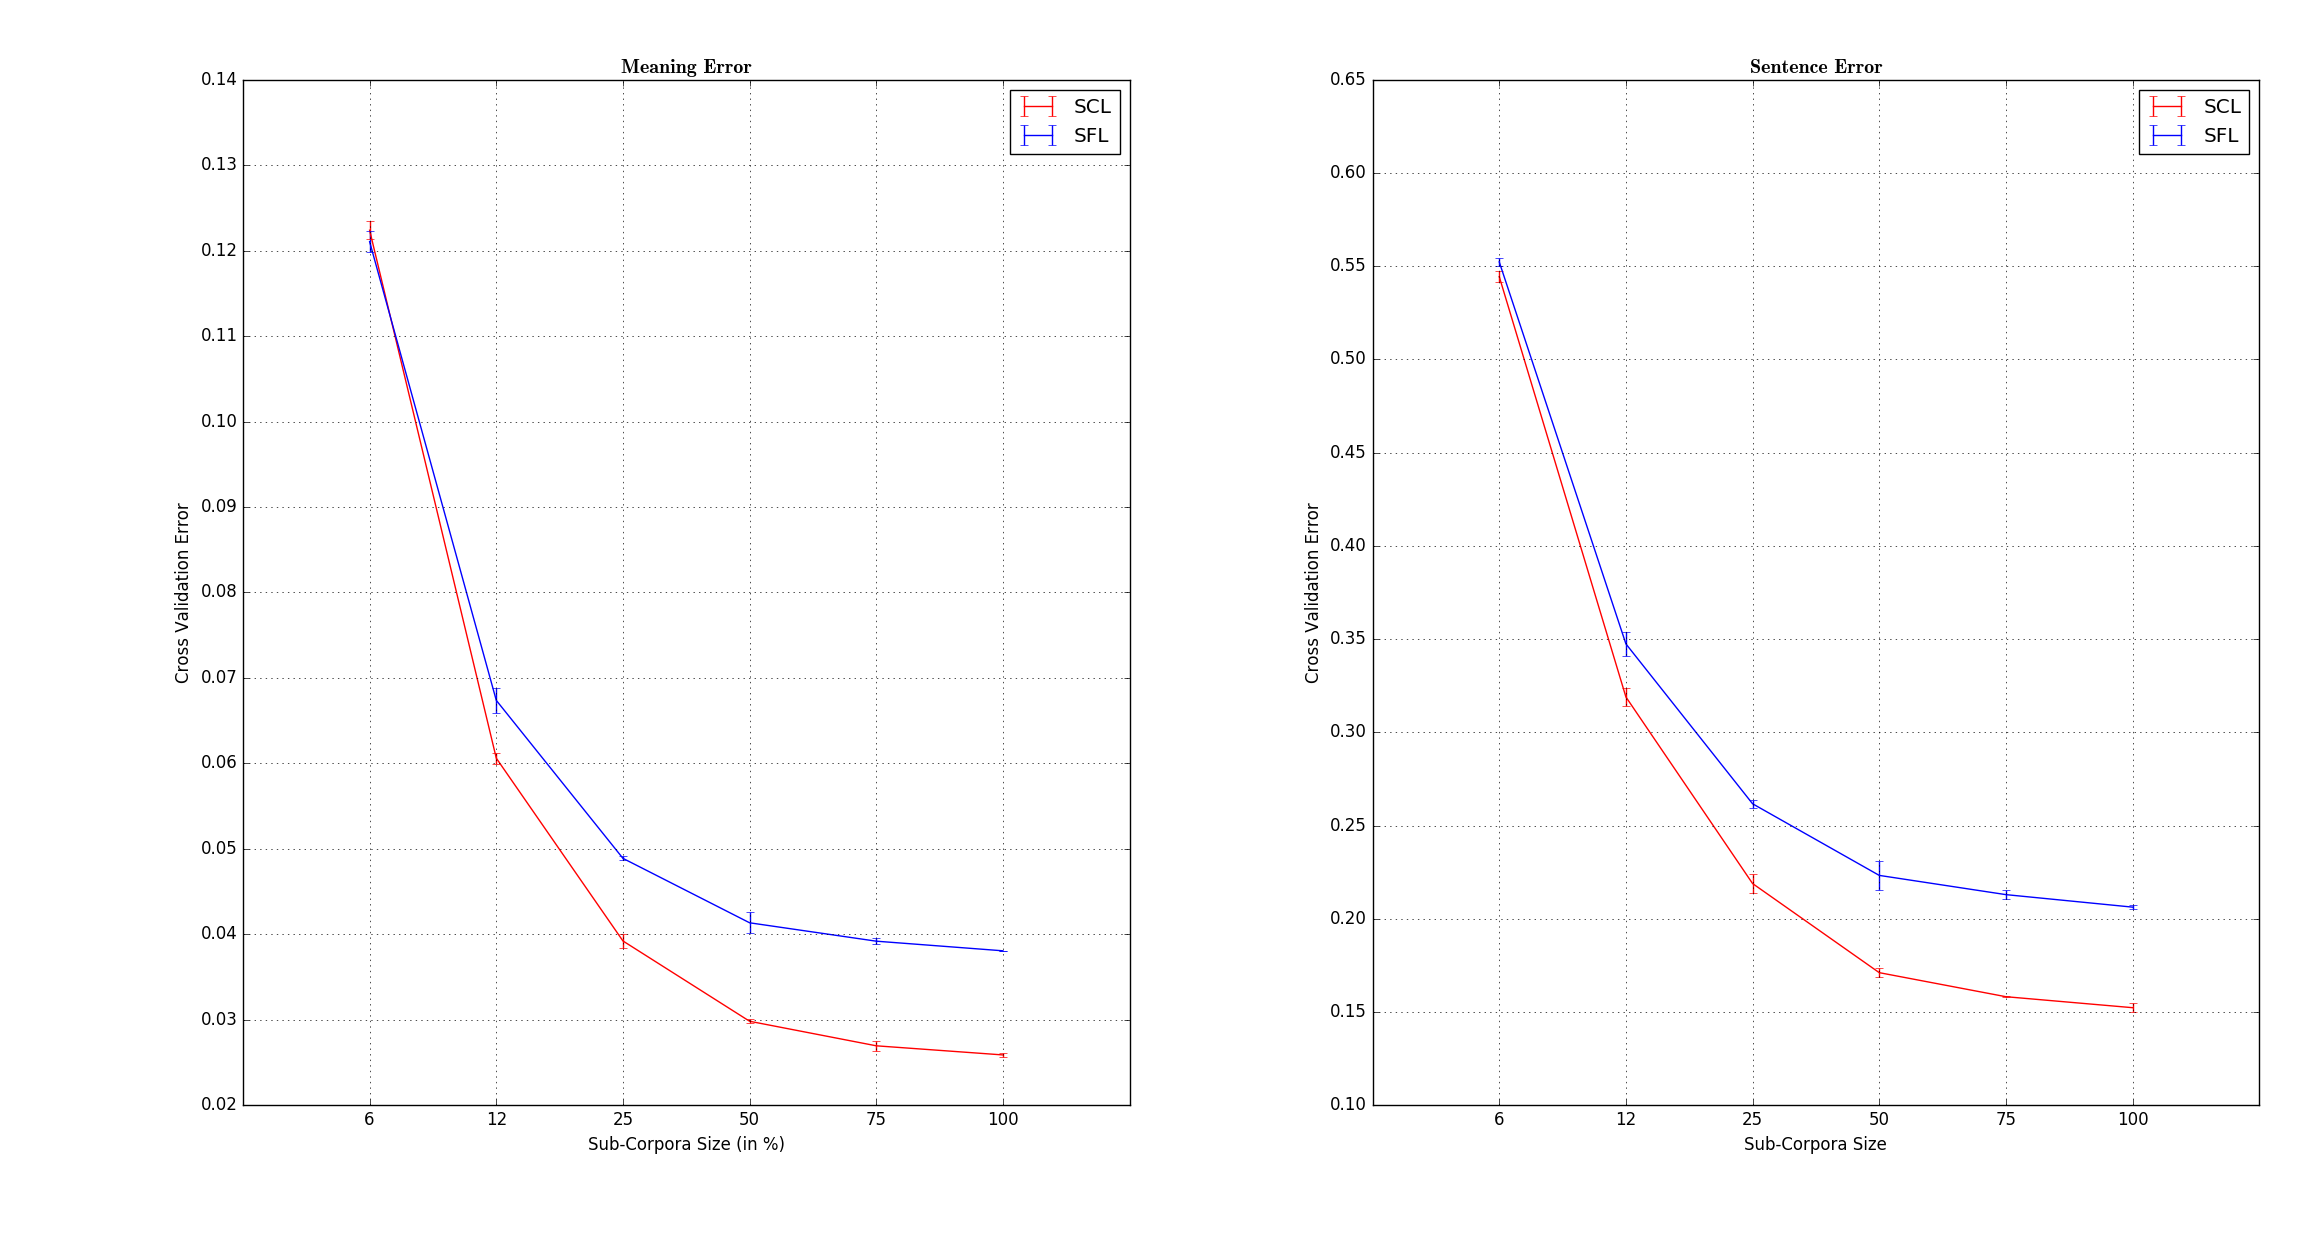
\includegraphics[width=1.0\linewidth]{corpus_size_1}
\caption[Effect of corpus size on Word2Vec-$\theta$RARes model.]{Effect of corpus size on cross validation errors of Word2Vec-$\theta$RARes model in SCL and SFL mode. NOTE: the scale of cross-validation error for the meaning and sentence error are different.}
\label{fig:corpus_size_1}
\end{figure}

Figure \ref{fig:corpus_size_1} shows the cross-validation errors rates with respect to corpus size on the Word2Vec-$\theta$RARes model. It can be observed that with the increase in corpus size from $6 \%$  to $50 \%$, the meaning error sharply drops from $12.18 \%$ to $2.96 \%$ in the SCL mode and from $11.96\%$ to $4.17 \%$ in the SFL mode. Similarly, the sentence error also decreases from $54.84 \%$ to $17.25 \%$ in SCL and from $54.14 \%$ to $22.41 \%$ in the SFL mode. When the sub-corpora size is $75\%$, where the model was trained only on $37.5\%$ of corpora size, the model already generalized with $2.72 \%$ meaning error and $15.98 \%$ sentence error in the SCL mode and with $3.95 \%$ meaning error and $21.33 \%$ sentence error in the SFL mode. Although the error rates gradually drop when the corpus size is further increased from $25\%$ to $100\%$ but the improvement rate of errors is very less. This indicates that cross-validation errors improve with the increase in corpus size up to a certain limit and any further increase in corpus size barely influence the performance of the model.

\begin{figure}[hbtp]
\centering
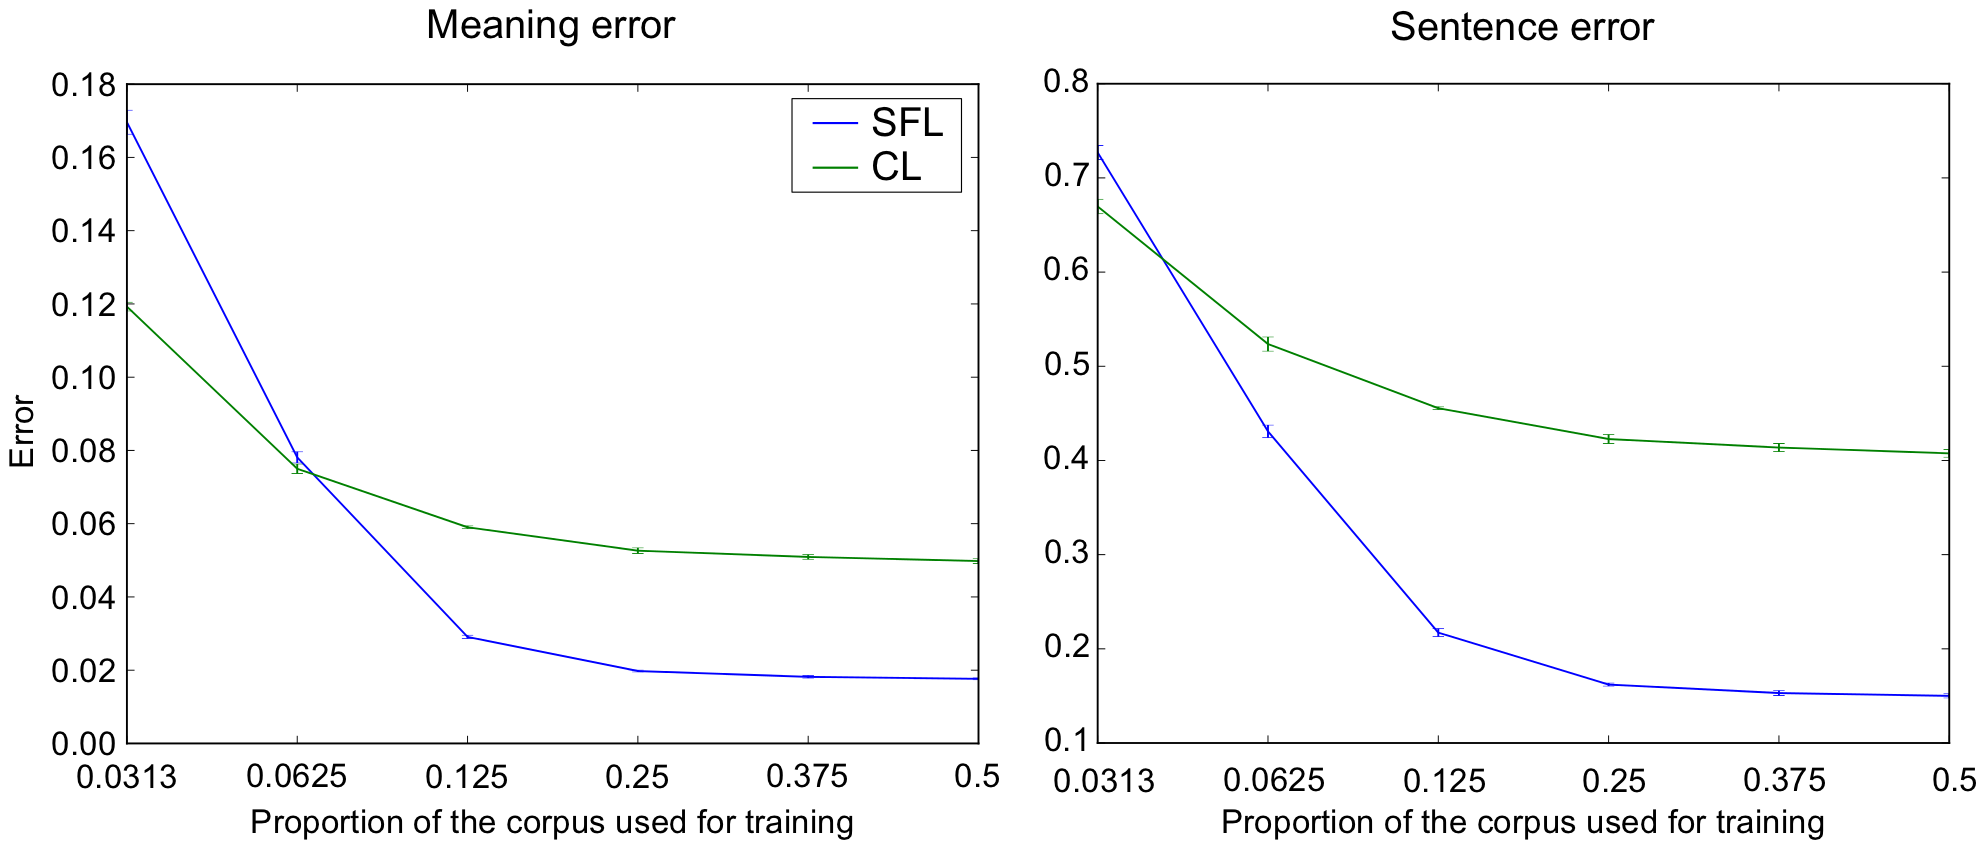
\includegraphics[width=1.0\linewidth]{corpus_size_xavier}
\caption[Effect of corpous size on $\theta$RARes model.]{Effect of corpus size on cross validation errors using $\theta$RARes model in SCL (legend CL) and SFL learning modes \cite{xavier:2013:RT}. NOTE: The x-axis represents the corpus-size used for training i.e. if sub-corpora size is $25\%$ then corresponding tick on the axis is 0.125 ($12.5\%$). The scale of cross-validation error for the meaning and sentence error are different.}
\label{fig:corpus_size_xavier}
\end{figure}

Comparing the effect of corpus size on Word2Vec-$\theta$RARes model (see fig. \ref{fig:corpus_size_1}) and the $\theta$RARes model (see fig. \ref{fig:corpus_size_xavier}), it can be observed that in SFL mode, with the increase in corpus size from $6\%$ to $25\%$, the meaning error in $\theta$RARes model dropped from $\approx 17\%$ to $\approx 3\%$ and the sentence error dropped from $\approx 70\%$ to $\approx 20\%$. Whereas in the Word2Vec-$\theta$RARes model, the meaning error dropped from $\approx 12\%$ to $\approx 5\%$ and the sentence error dropped from $\approx 55\%$ to $\approx 26\%$. Also, with the increase in corpus size further from $25 \%$, the cross-validation errors asymptotes in both the models with negligible improvement in error rates. Overall, with the increase in corpus size, the improvement in error rates with $\theta$RARes model in the SFL mode is higher as compared to Word2Vec-$\theta$RARes model.

Comparing the performance of both the $\theta$RARes and Word2Vec-$\theta$RARes model in the SCL mode, it can be seen that the meaning error in latter continuously drops when the corpus size is further increased from $12 \%$ whereas in the $\theta$RARes model the decline in meaning error is negligible. The sentence error in $\theta$RARes model drops by a small amount when corpus size is increased from $6 \% $ to $25 \%$, but asymptotes as the corpus size is further increased from $25\%$ whereas, it gradually drops in Word2Vec-$\theta$RARes model. From the lower to the upper limit of corpus size studied, the sentence error with the  $\theta$RARes model in SCL mode dropped from $\approx 65\%$ to $\approx 40\%$ whereas, in the Word2Vec-$\theta$RARes model it dropped from $\approx 55\%$ to $\approx 15 \% $. The meaning error in SCL mode, on the other hand, dropped from $\approx 12\%$ to $\approx 5\%$ in the $\theta$RARes model whereas, in the Word2Vec-$\theta$RARes model it dropped from $\approx 12\%$ to $\approx 2\%$.

Overall, in SCL mode, it can be seen that on the range of sub-corpora size investigated in the experiment, the Word2Vec-$\theta$RARes model performed better than $\theta$RARes model with all sub-corpora sizes. Whereas in SFL mode, the $\theta$RARes model performs better than Word2Vec-$\theta$RARes model. Another pattern which can be observed is that with all sub-corpora sizes, the Word2Vec-$\theta$RARes model performs better in the SCL mode than the SFL mode. Whereas in the $\theta$RARes model, with the increase in corpus size the model performs better in SFL model than SCL mode. 

\section{Experiment-6: Generalization on New Corpus}

One may argue that the previously used corpora (corpus-462 and corpus-90582), were artificially constructed using context-free grammar and may add a bias to the model, thus making it easier for the model to learn and generalize on these corpora for the TRA task. To answer this question, in this experiment, the corpus-373 containing the instructions collected from human participants in a Human-Robot Interaction (HRI) study of language acquisition (as discussed in section \ref{corpora}) was used.

\paragraph{Word2Vec-$\theta$RARes model:} To test the generalization of Word2Vec-$\theta$RARes model on corpus-373, the model was operated in SCL mode and tested using the LoO cross-validation method. The SCL mode and the LoO method were chosen so that the results of this experiment can be compared with that of obtained using $\theta$RARes model \cite{tra:xavier_hri}. Also, to make the results of both the model deterministically comparable, topologically modified coding was not utilized for this experiment (see section \ref{sec:w2v-esn_model}) and simulations were performed using ten reservoir instances. For this experiment, reservoir parameter space was not explored to identify the optimal reservoir parameters, instead, the previously optimized parameters obtained on corpus-462 with topological modified coded meaning was used i.e. $SR = 2.4$, $IS = 2.5$ and $LR = 0.07$ (see section \ref{grid_search}). Doing so will also enable us to test the robustness of these model parameters on the new corpus i.e. corpus-373.

Table \ref{tab:corpus_373} reports the mean sentence error and best generalization error values obtained with the Word2Vec-$\theta$RARes and $\theta$RARes model. The best generalization error here represents the percentage of sentences whose meanings were predicted incorrectly in common by all 10 model instances \cite{tra:xavier_hri}. In comparison to the $\theta$RARes model, the mean sentence error in the Word2Vec-$\theta$RARes model improved by $26.31\%$ and $17.97\%$  with the reservoir of size 500 and 1000 respectively. The best generalization errors also improved by $17.96 \%$ and $9.12 \%$ with the reservoir size 500 and 1000 respectively.

The Word2Vec-$\theta$RARes model generalized better with both the reservoir sizes (500 and 1000) as compared to the $\theta$RARes model. Notice the improvement in both the models with the increase in reservoir size from 500 to 1000 neurons. It can be seen that the improvement in cross-validation error in the Word2Vec-$\theta$RARes model is comparatively less than the $\theta$RARes model. With the increase in reservoir size from 500 to 1000, the mean sentence error and the best generalization error in $\theta$RARes improved by $10.7 \%$ and $9.65 \%$ respectively. Whereas with the Word2Vec-$\theta$RARes model, the mean sentence error and the best generalization error improved by $2.36 \%$ and $0.81\%$ respectively. This suggests that the generalization ability of the Word2Vec-$\theta$RARes model on corpus-373 is negligibly affected by the increase in reservoir size.  

\begin{table}
\centering
\begin{threeparttable}
\caption[Word2Vec-$\theta$RARes model generalizing on new corpus]{Generalization error in SCL mode on corpus-373.}
\label{tab:corpus_373}
\rowcolors{2}{gray!25}{white}
\begin{tabular}{llcc}
\hiderowcolors
\toprule
Reservoir              &  Error     &   Word2Vec-$\theta$RARes Model        & $\theta$RARes Model \\
\midrule
\showrowcolors                 
\textbf{500 N}    & mean (std.)         & 42.65 ($\pm$ 1.36)     & 68.96 ($\pm$ 2.03)  \\
                    & Best             & 26.54                 & 44.50  \\
\textbf{1000 N}    & mean (std.)         & 40.29 ($\pm$ 1.13)     & 58.26 ($\pm$ 1.37)\\
                    & Best             & 25.73                 & 34.85 \\
\bottomrule
\end{tabular}
\begin{tablenotes}
\small
\item 
Sentence and best generalization errors (in $\%$) obtained with the Word2Vec-$\theta$RARes model and the $\theta$RARes in SCL mode with reservoir of 500 and 1000 neurons. The results reported are mean and standard deviation of errors obtained with 10 model instances. The best generalization error here means the percentage of sentences predicted incorrectly in common by all 10 reservoir instances \cite{tra:xavier_hri}.
\end{tablenotes}
\end{threeparttable}
\end{table} 

Figure \ref{fig:373_stats_500} and \ref{fig:373_stats_1000} shows the number of erroneous sentences by number of model instances with reservoir size 500 and 1000 respectively. With a reservoir of 500 neurons (see fig. \ref{fig:373_stats_500}), all the ten instances of Word2Vec-$\theta$RARes and $\theta$RARes model correctly predicted the meaning of 146 and 35 sentences respectively. Whereas the meaning of 99 and 166 sentences out of 373 was wrongly predicted by all the ten instances of Word2Vec-$\theta$RARes and $\theta$RARes model. 

\begin{figure}[hbtp]
\centering
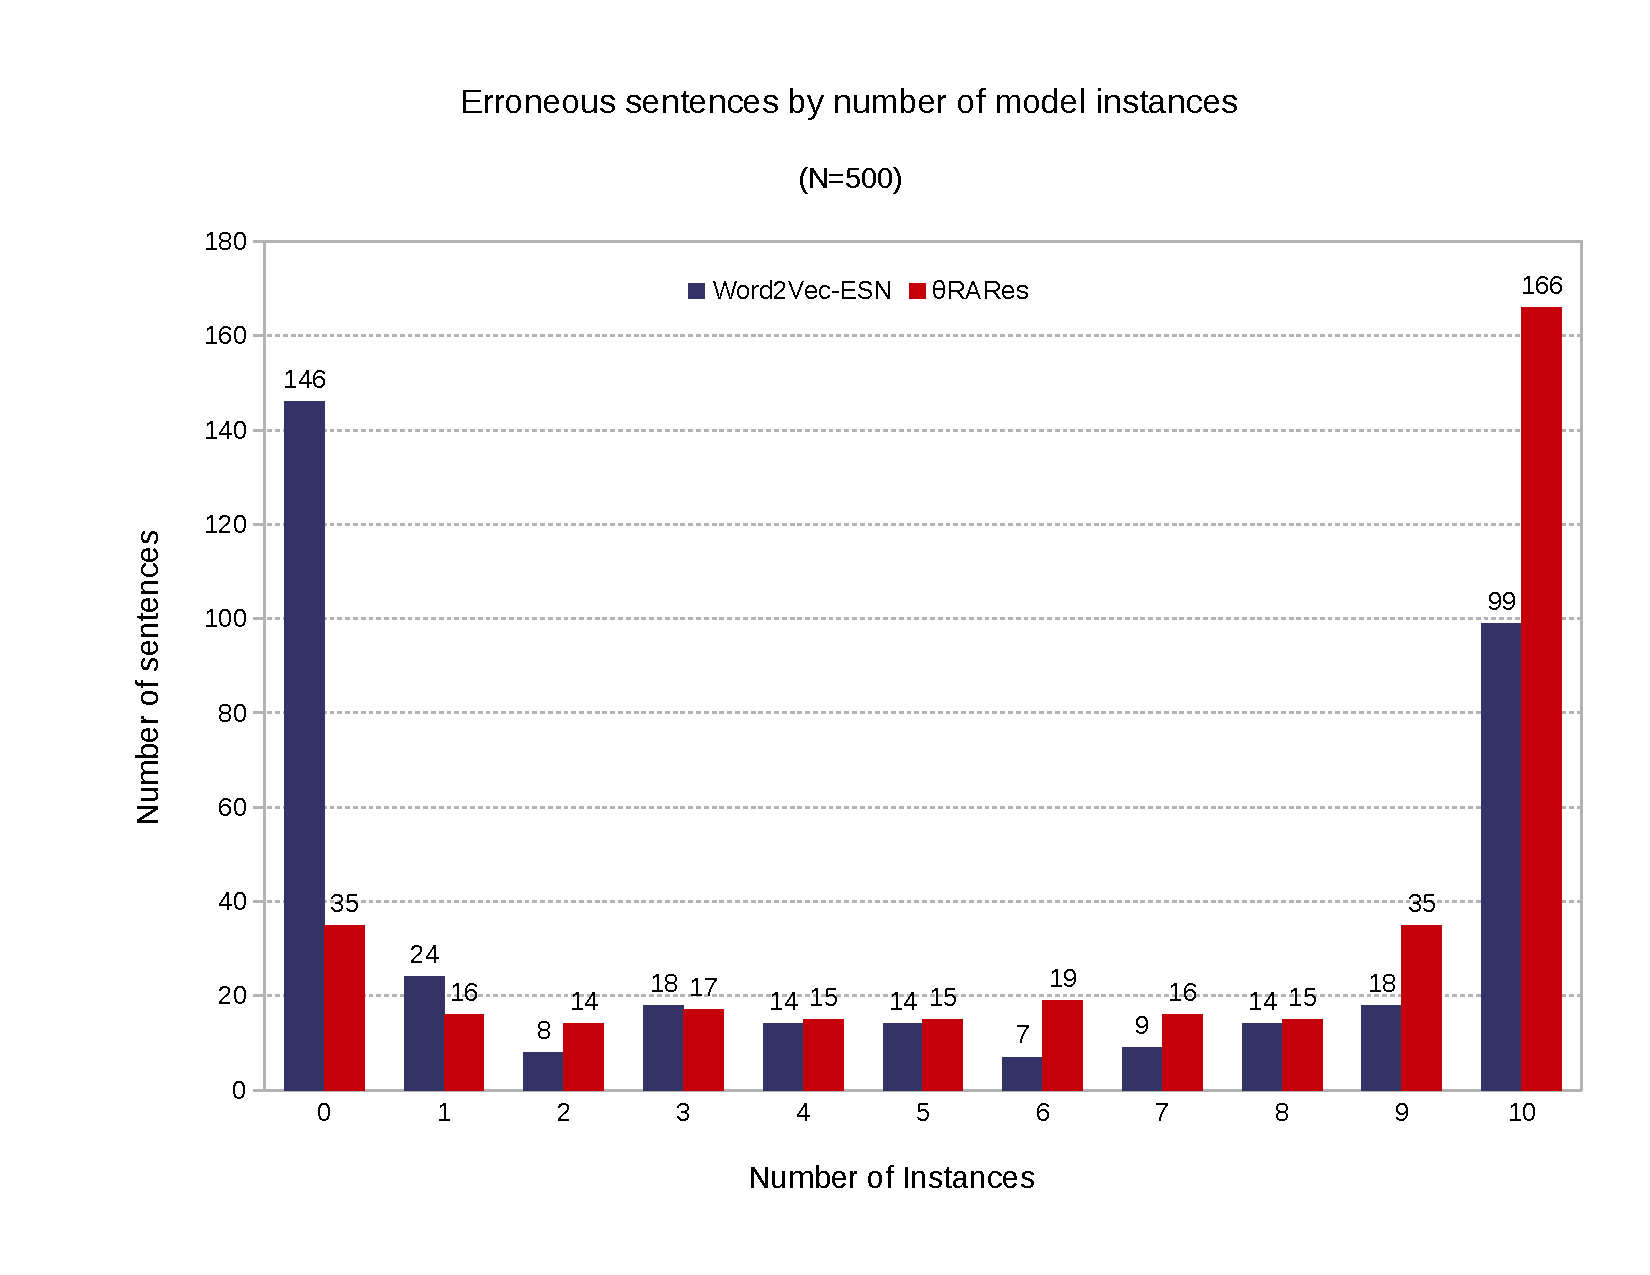
\includegraphics[width=0.9\linewidth]{500_res}
\caption[Sentence error count by number of model instances with reservoir size 500.]{Sentence error count by number of instances with reservoir of 500 neurons.}
\label{fig:373_stats_500}
\end{figure}

\begin{figure}[hbtp]
\centering
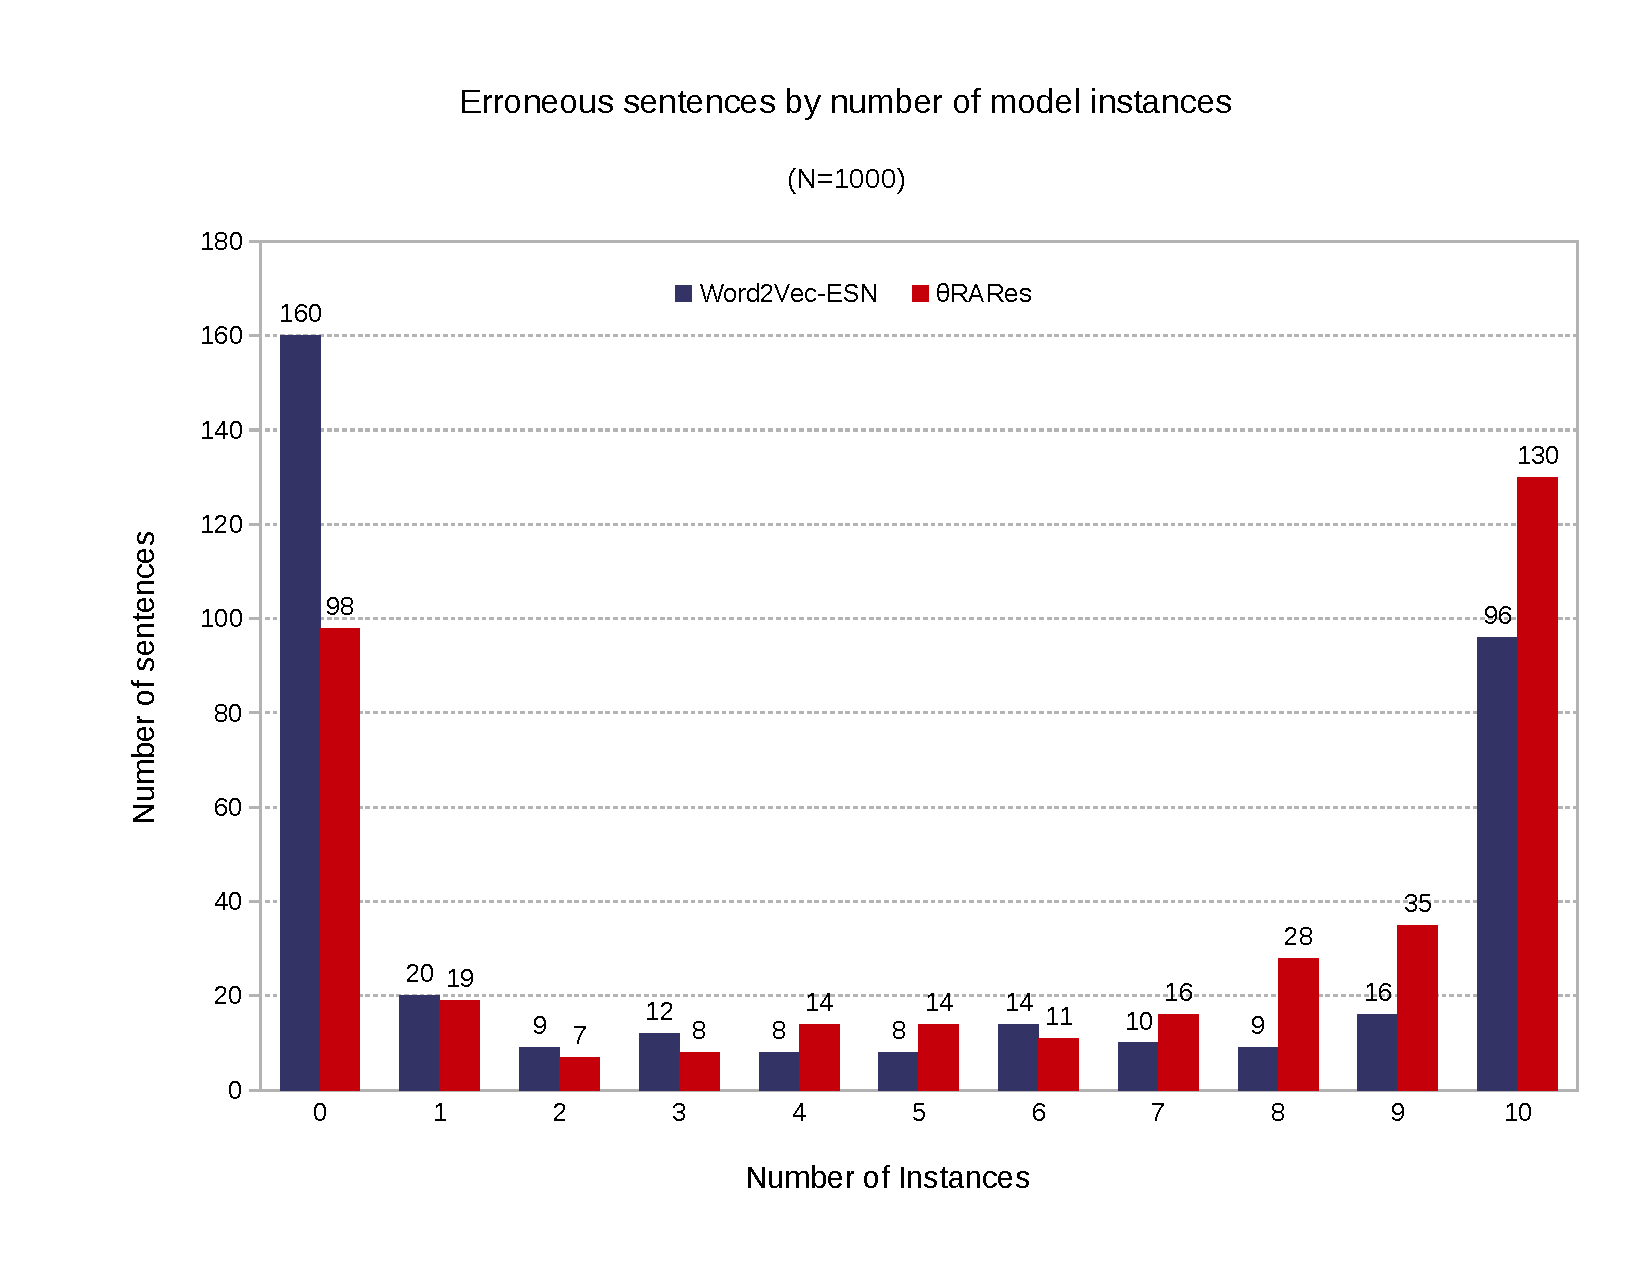
\includegraphics[width=0.9\linewidth]{1000_res}
\caption[Sentence error count by number of model instances with reservoir size 1000.]{Sentence error count by number of model instances with reservoir of 1000 neurons.}
\label{fig:373_stats_1000}
\end{figure}

With the increase in the reservoir from 500 to 1000 neurons, the number of sentences correctly predicted by all the instances of Word2Vec-$\theta$RARes and $\theta$RARes model increased respectively from 146 to 160 and from 35 to 98. Also, the count of sentences where all model instances failed to predict the meaning correctly dropped from 99 to 96 and 166 to 130 for Word2Vec-$\theta$RARes model and $\theta$RARes model respectively. Notice that with both the reservoir sizes, the number of sentences whose meanings were correctly predicted by all the model instances of Word2Vec-$\theta$RARes model is higher than the $\theta$RARes model. Whereas the count of sentences wrongly predicted by all model instances is lower in Word2Vec-$\theta$RARes model as compared to that of $\theta$RARes model.

\section{Experiment-7: Effect of Word2Vec Word Dimensions}

In all the previous experiments, the distributed word vectors of 50 dimensions were used. However, Mikolov et al. \cite{w2v:mikolov_2013_efficient, w2v:mikolov_2013_distributed} showed that the word vectors of higher dimensions (e.g. 300 in their case) perform better on word analogy task. Thus in this experiment, the effect of distributed word vector dimensions on the TRA task will be explored.

\paragraph{Word2Vec-$\theta$RARes model:} Recall that in section \ref{get_word_embeddings}, six Word2Vec models were trained to generate the word vectors of 20, 30, 50, 100, 200, 300 dimensions respectively. To test the effect of these word vector dimensions on the TRA task, each of these Word2Vec models was used with the Word2Vec-$\theta$RARes model. For this experiment, the sentences of corpus-373 without the topologically modified coded meaning were used (see fig. \ref{fig:model_variant_1}). Simulations were performed using ten model instances each with a reservoir of 1000 neurons. The model was trained and tested using LoO cross-validation approach in both the SCL and SFL mode, and all the reservoir parameters were kept identical to Experiment-2.

\begin{figure}[hbtp]
\centering
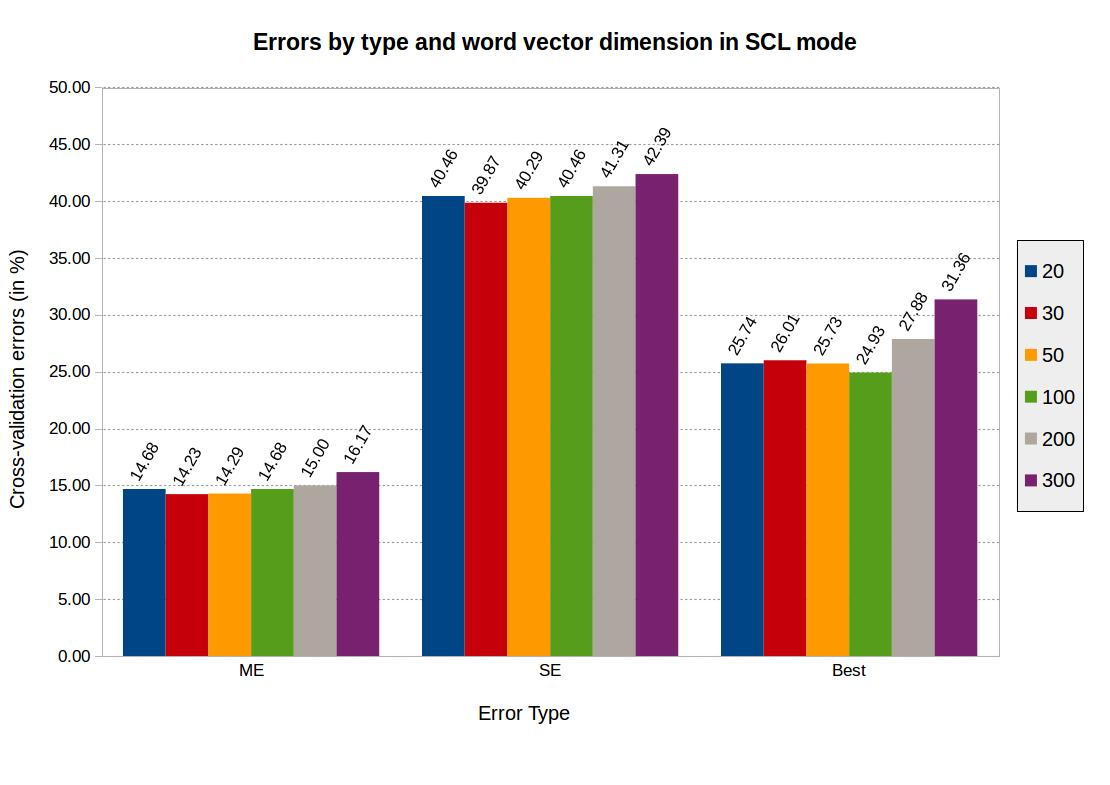
\includegraphics[width=0.9\linewidth]{word_dim_scl}
\caption[Effect of word vector dimensions on Word2Vec-$\theta$RARes model in SCL mode.]{\textbf{Effect of word vector dimensions on cross validation errors of Word2Vec-$\theta$RARes model in SCL mode: } {\small Cross-validation error are given in percentage. Error type includes ME: Meaning Error, SE: Sentence error, Best: Best generalization error.}}
\label{fig:word_dim_scl}
\end{figure}

\begin{figure}[hbtp]
\centering
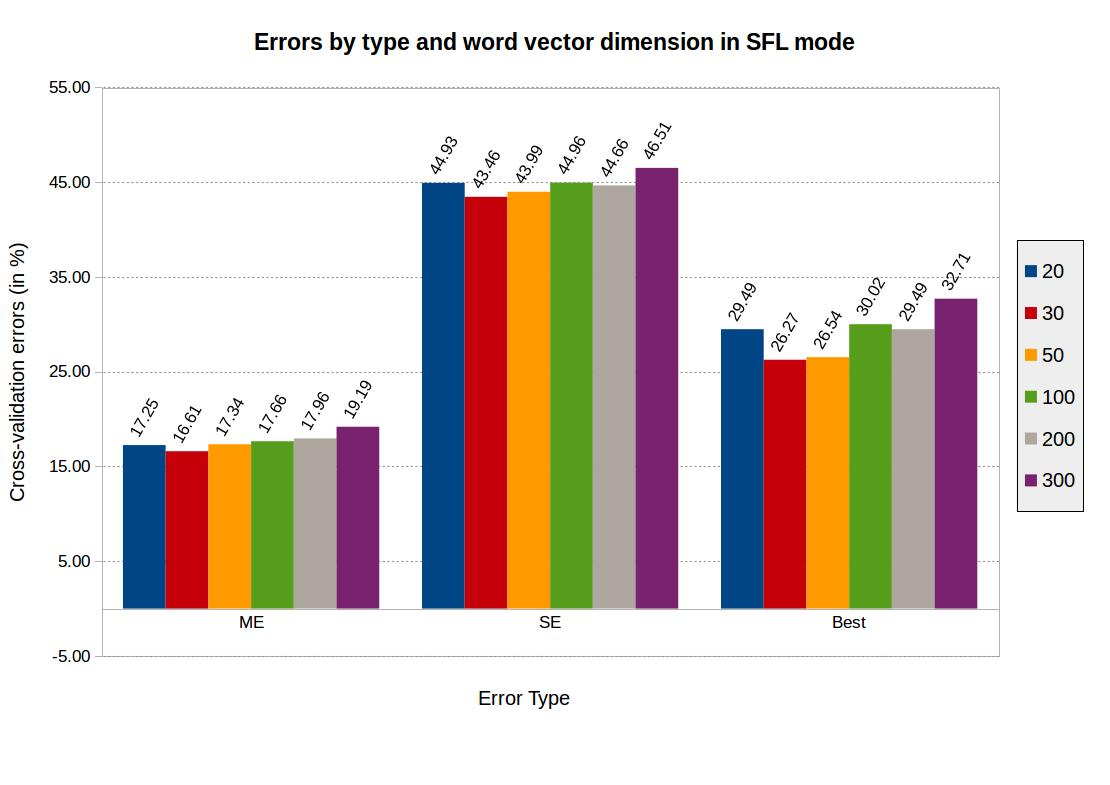
\includegraphics[width=0.9\linewidth]{word_dim_sfl}
\caption[Effect of word vector dimensions on Word2Vec-$\theta$RARes model in SFL mode.]{\textbf{Effect of word vector dimensions on cross validation errors of Word2Vec-$\theta$RARes model in SFL mode: }{\small Cross-validation errors are given in percentage. Error type includes ME: Meaning Error, SE: Sentence error, Best: Best generalization error.}}
\label{fig:word_dim_sfl}
\end{figure}

Figure \ref{fig:word_dim_scl} and \ref{fig:word_dim_sfl} shows the effect of word vector dimensions on the cross-validation errors of Word2Vec-$\theta$RARes model in SCL and SFL mode respectively. The corresponding errors are also reported in Table \ref{tab:word-vector-size}. In the figures, we can see that from lower to the upper limit of the word vector dimensions studied, all the error measures in both the learning modes increased approximately by $2\%$. Also, in the range of 20 to 200 dimensions, the cross-validation errors remained almost equivalent with negligible fluctuations. The minimum errors were obtained with word vectors of 30 dimensions i.e. $ME= 14.23$, $SE= 39.87$ in the SCL mode and $ME= 16.61$, $SE= 43.46$ in the SFL mode. Another interesting pattern which can be observed is that with all the word vector dimensions, the model in SCL mode always performed better as compared to SFL mode. The similar relation between SCL and SFL mode was also observed in the previous experiments as well. Overall, it was observed that the word vectors dimensions have a negligible effect on the performance of Word2Vec-$\theta$RARes model for the TRA task.

\section{Neural Output Activity of the Word2Vec-$\theta$RARes Model}

In the previous experiments, we observed that the cross-validation error rates dropped with the increase in corpus size. So, the 45 sentences of corpus-45 were added to corpus-462 to get the resultant corpus have 507 sentences (462 + 45). The readout activations of the Word2Vec-$\theta$RARes model were then analyzed for the sentences in the newly formed corpus of 507 sentences and corpus-373. This analysis of readout activation will allow us to have an insight on how the model is processing the distributed word vectors to generate the meaning of the sentences. It was observed that the model is re-analyzing the thematic roles of the input sentences across the time. The same behavior was also pointed out by Hinaut et. al \cite{tra:xavier_hri, xavier:2013:RT} with $\theta$RARes model.

\subsection{Output activity for sentences with topologically modified coded meaning}

Figure \ref{fig:act_analysis_1} shows the read out activations of the second noun in the following four sentences across time. Note that the sentences \ref{activation:sent-1} and \ref{activation:sent-2} are active constructions whereas \ref{activation:sent-3} and \ref{activation:sent-4} are passive constructions.

\begin{enumerate}[noitemsep]
\item The man \textit{gave}(V1) the \textit{book}(N2) to the boy. \label{activation:sent-1}
\item The man \textit{took}(V1) the \textit{ball}(N2) that \textit{hit}(V2) the glass. \label{activation:sent-2}
\item The boy \textit{caught}(V1) the \textit{ball}(N2) that was \textit{thrown}(V2) by the man.  \label{activation:sent-3} 
\item The ball was \textit{pushed}(V1) by the \textit{man}(N2).  \label{activation:sent-4}
\end{enumerate}

\begin{figure}[hbtp]
\centering
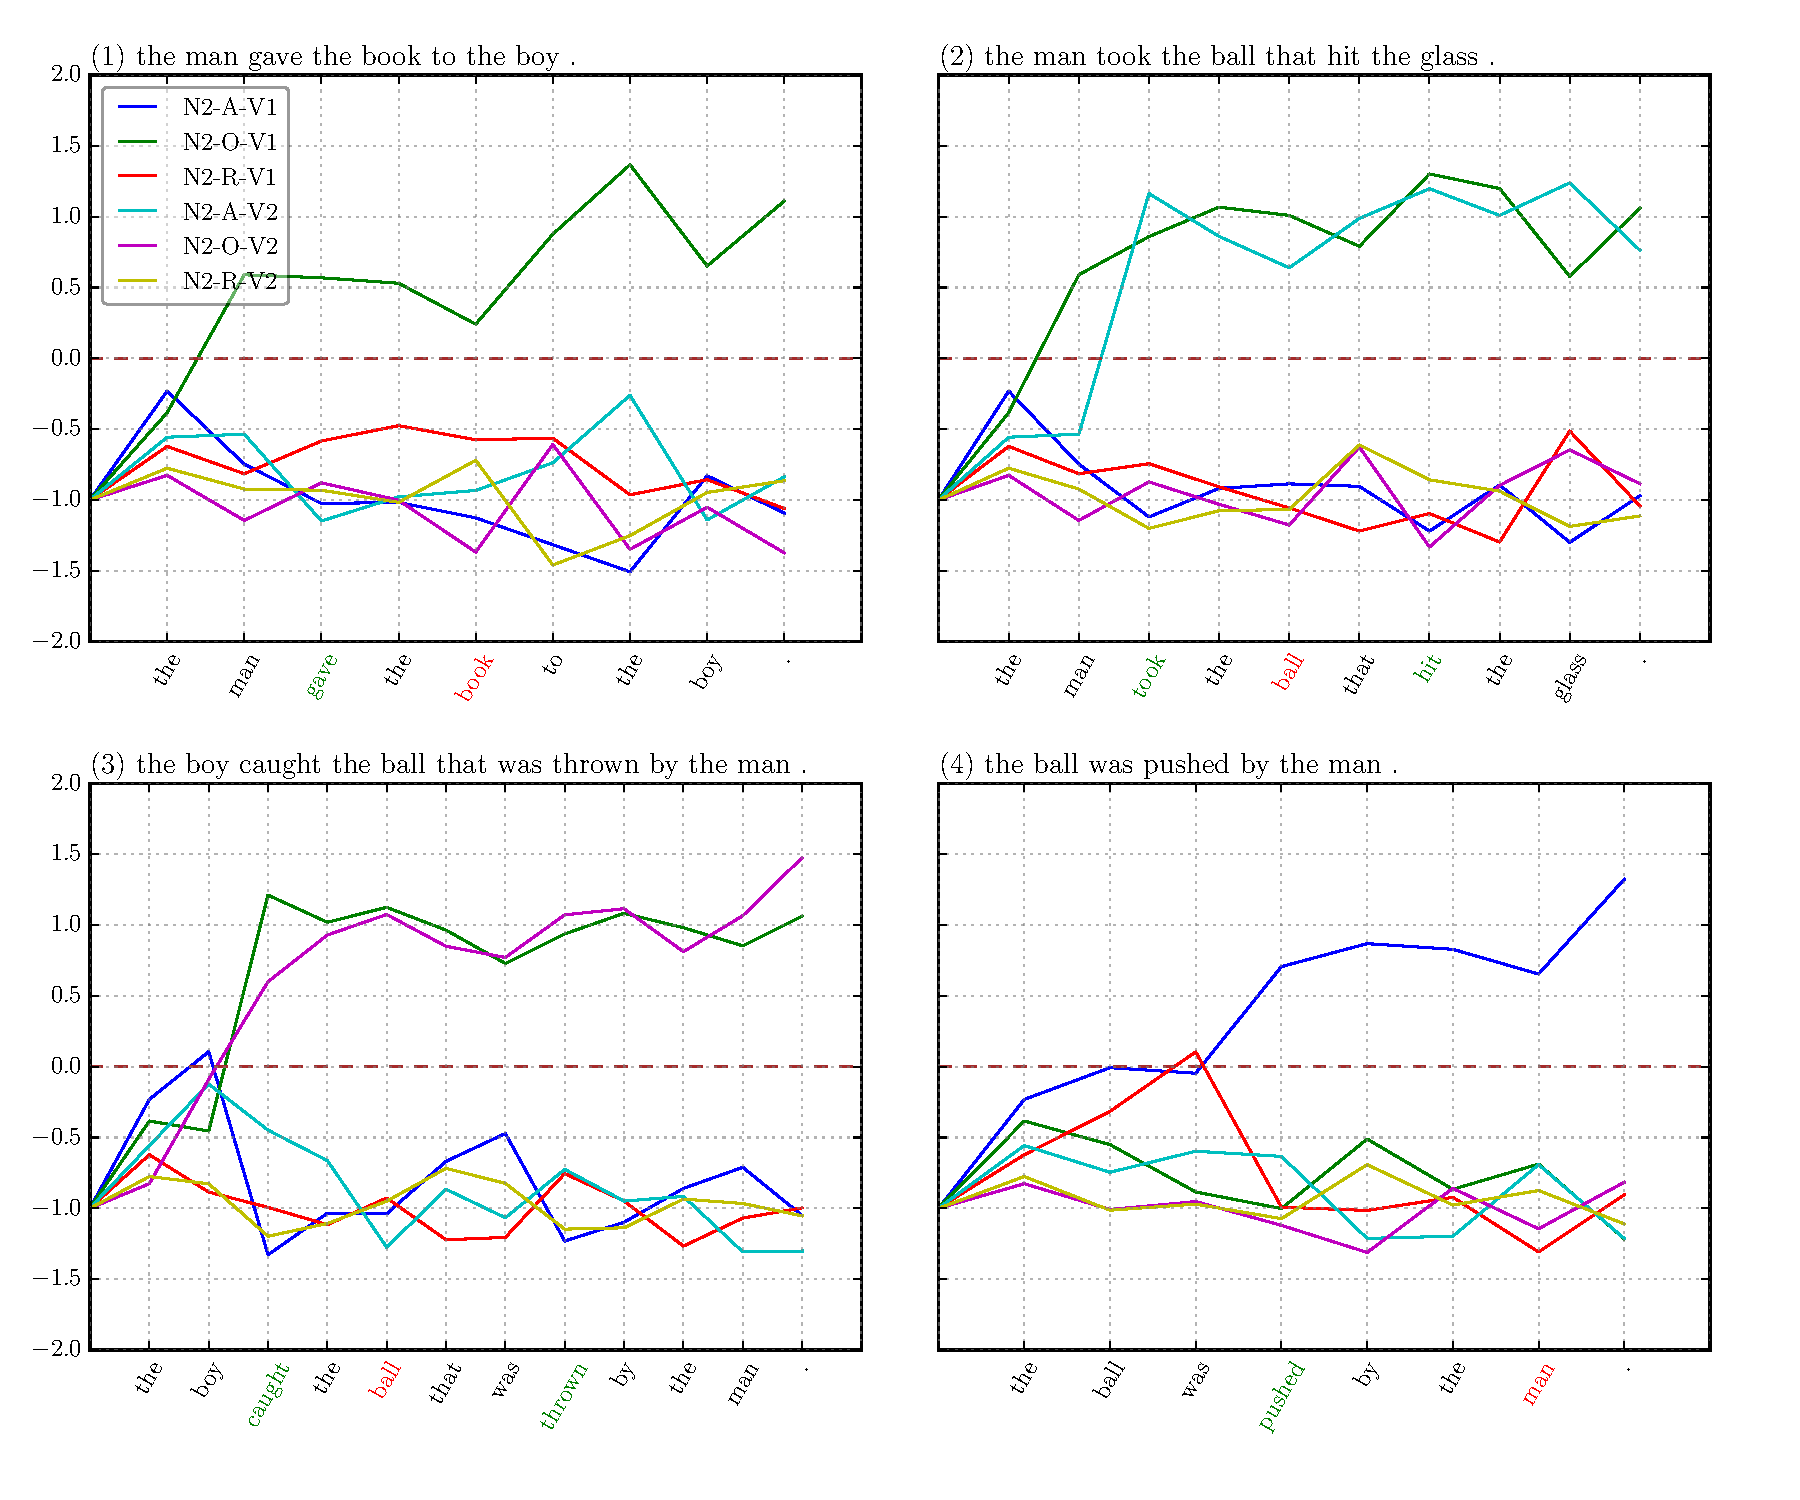
\includegraphics[width=1.0\linewidth]{act_analysis_1}
\caption[Readout activity of Word2Vec-$\theta$RARes model for a sentence with topologically modified coded meaning.]{\textbf{Readout activity of Word2Vec-$\theta$RARes model for a sentence with topologically modified coded meaning: } {\small Each coloured line shows the thematic role of Noun-2 (tick marked in red) with respect to Verb-1 and Verb-2 (ticks shown in green).}}
\label{fig:act_analysis_1}
\end{figure}

Each colored line in the graph (see fig. \ref{fig:act_analysis_1}) represents the possible thematic roles of the second noun (N2) which can have one of the three possible roles i.e. Agent (A), Object (O) or Recipient (R), with respect to either Verb-1 (V1) or Verb-2 (V2). N2 is marked in red and verbs are marked in green on the x-axis. In the figure, the role `N2-A-V1' can be interpreted as the second noun (N2) is the agent of the first verb (V1). 

As all the four sentences start with `the', the activations at this word is same for all four sentences. With the introduction of the first noun (`man') in sentences \ref{activation:sent-1} and \ref{activation:sent-2}, the readout activations of role N2 as object of V1 (N2-O-V1) goes above the threshold 0. Thus the model predicts that the N2 could be the object of V1. In sentence \ref{activation:sent-3}, with the arrival of the first noun (`boy'), the competition between roles N2-A-V1, N2-A-V2, and N2-O-V2 can be seen, but only the role N2-A-V1 (agent of verb `caught') managed to cross the threshold. Whereas, in sentence \ref{activation:sent-4}, the activation of role N2-A-V1 is higher when the first noun (`ball') is encountered, but with the arrival of `was' the role of N2 is changed as recipient of V1 (`pushed').

In sentence \ref{activation:sent-1}, the activation of role N2-A-V1 is maintained, and no other role managed to cross the threshold with the arrival of V1 (`gave')
Whereas in sentence \ref{activation:sent-2}, with the advent of the V1 (`took') the activation for N2-A-V2 goes above threshold, indicating the presence of V2 (`hit') in the sentence even before the model has encountered the second verb. In sentence \ref{activation:sent-3} and \ref{activation:sent-4}, with the arrival of V1 (`caught' and `pushed' respectively) one can notice the re-analysis made by the model. In sentence \ref{activation:sent-3}, the activation of N2-A-V1 goes below the threshold and takes the new role as the object of both V1 (`caught') and V2 (`thrown'), i.e., N2-O-V1 and N2-O-V2. In sentence \ref{activation:sent-4}, the previously predicted role N2-R-V1 goes below the threshold with the arrival of V1 (`pushed').

Throughout the rest of sentence \ref{activation:sent-1}, the prediction N2-O-V1 is maintained with some minor ups and downs. Similarly, in sentence \ref{activation:sent-2}, the predictions of N2 alternates between roles N2-O-V1 and N2-A-V2 but the activation of both the roles remains above the threshold. In sentence \ref{activation:sent-3} the model sees both N2-O-V1 and N2-O-V2 as the preferred predictions, both being almost with similar activations and only alternating slightly. In sentence \ref{activation:sent-4}, the prediction of role N2-A-V1 do not change again throughout the sentence ever since the arrival of V1 (`pushed').

It can be seen that, at the end of the sentences, the model predicted the meaning of all the four sentences correctly. Also, notice the early prediction of correct roles even before the sentence is completed. The distributed representation of words learned from the nearby words and possibly encapsulating the information about them can be credited for such behavior.

\subsection{Output activity for sentences without topologically modified coded meaning} 

Figure \ref{fig:act_analysis_2} shows the readout activations of the following two sentences taken from corpus-373. 

\begin{enumerate}[noitemsep,label=(\Alph*) ]
\item \textit{put}(X1) the \textit{cross}(X2) on my \textit{right}(X3) \label{activation:sent-a}
\item \textit{push}(X1) the \textit{triangle}(X2) to the \textit{left}(X3) then \textit{push}(X4) the \textit{cross}(X5) to the \textit{left}(X6) \label{activation:sent-b}
\end{enumerate}

\begin{figure}[hbtp]
\centering
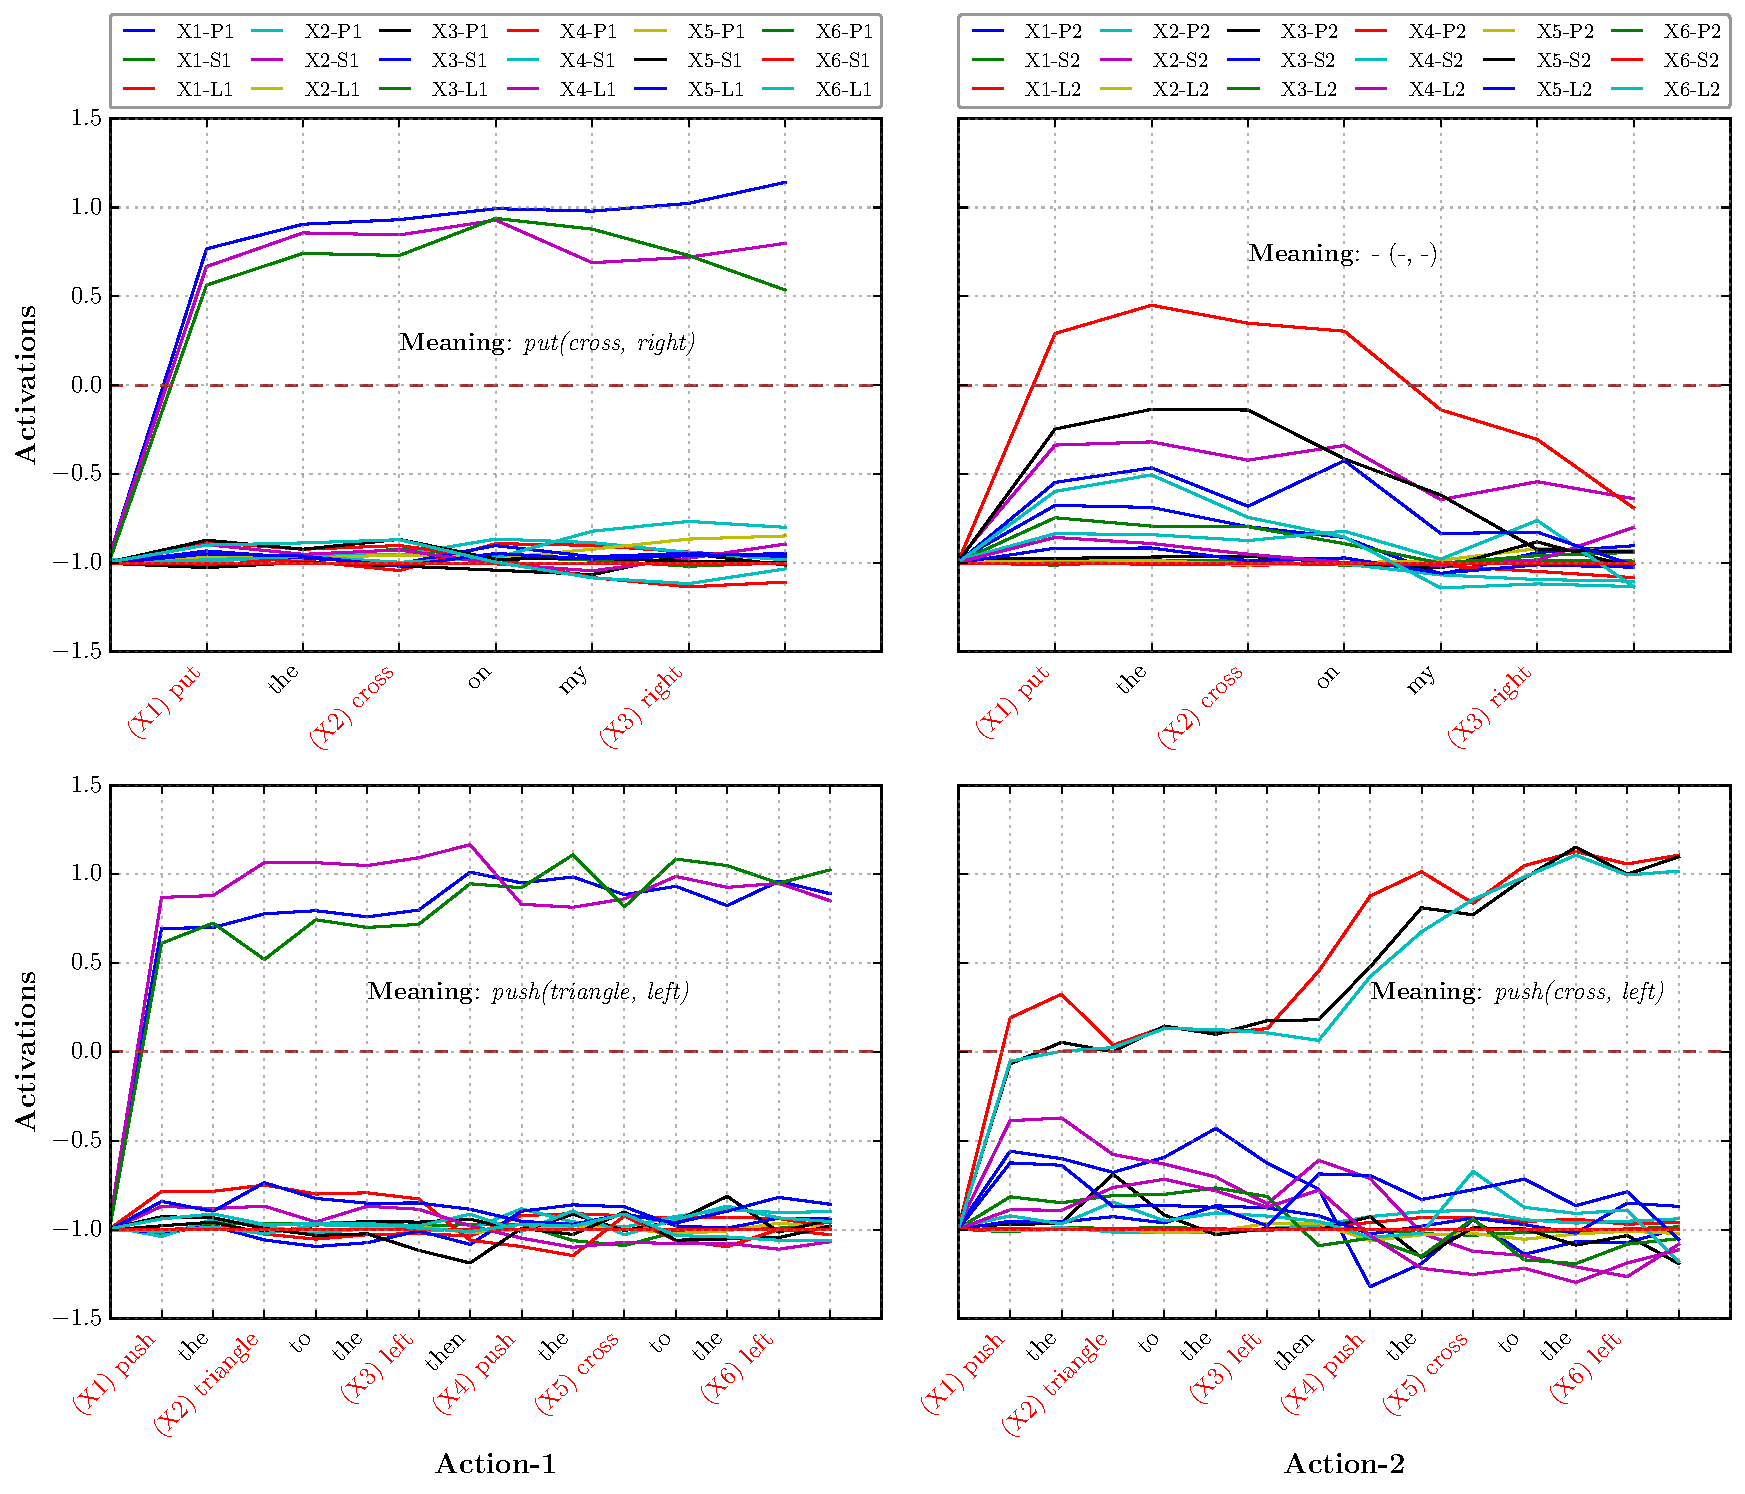
\includegraphics[width=1.0\linewidth]{act_analysis_2}
\caption[Readout activity of Word2Vec-$\theta$RARes model for a simple and complex sentence from corpus-373.]{\textbf{Readout activity of Word2Vec-$\theta$RARes model for a simple and complex sentence from corpus-373: }{\small First and second row shows the readout activation for a simple and complex sentence respectively. Each column in the figure shows the activation of the corresponding sentence with respect to an action.} }
\label{fig:act_analysis_2}
\end{figure}

Note that the sentence \ref{activation:sent-a} is a simple instruction to perform only one action and contains three semantic words (X1-X3). Whereas sentence \ref{activation:sent-b}, is a complex instruction to perform two actions and contains six semantic words (X1-X6). Each semantic word in the sentences can have a role with respect to a maximum of two actions (see corpus-373 in section \ref{corpora}). A role X1-P1, for example, is interpreted as the first semantic word (X1)  is the predicate of action-1. The roles predicate, subject and location are represented by `P', `S' and `L' respectively.

The first row of Figure \ref{fig:act_analysis_2} shows the readout activity of the model for sentence \ref{activation:sent-a} with respect to action-1 (left) and action-2 (right). One can see that for action-1, the model correctly predicts the meaning \textit{put(cross, right)}, whereas for the action-2, at the end of sentence all the neural activations go below the threshold 0. Thus, this indicates the presence of only action-1 in the sentence  \ref{activation:sent-a}. Also, for the action-2, notice the online re-analysis behavior of the model where the activation of role (X1-L2) goes above the threshold 0 at the beginning of the sentence but later drops below the threshold at the end of the sentence.

The second row of Figure \ref{fig:act_analysis_2} illustrates the readout activity of sentence \ref{activation:sent-b} for each action. The model correctly predicts the thematic roles of constituent semantic words (X1 to X6) for both the actions. For the action-1, the model makes early predictions of roles i.e. \textit{push (triangle, left)}, whereas, for action-2, the activation of correct roles are reinforced when the model encounters the second predicate (X4 = `push') in the sentence. Thus the model predicts the meaning of sentence for the second action as \textit{push (cross, left)}.

\section{Comparative Analysis of Sentences Meaning}

In the previous section, we saw the online re-analysis of sentences with and without the topologically modified coded meanings by the Word2Vec-$\theta$RARes model. So far, we have also seen the performance of Word2Vec-$\theta$RARes model in numbers. In this section, we will analyze for what type of sentences the Word2Vec-$\theta$RARes model correctly predicted the meanings, but the $\theta$RARes model failed. Also, we will see the kind of sentences for which the Word2Vec-$\theta$RARes model failed to predict the meaning correctly. This analysis was done on the results obtained in Experiment-6 using corpus-373.

While analyzing the sentences whose meanings were correctly predicted by all ten instances of the Word2Vec-$\theta$RARes model and incorrectly predicted by the $\theta$RARes model, a significant number of patterns were identified. Almost $85 \%$ of the sentences whose meaning were wrongly predicted by all the instances of $\theta$RARes model were either two action commands or redundant commands (see fig. \ref{fig:meaning_realtions}). For example, ``push the circle in the middle and put it in the right" and ``push the circle to the middle and then put it on the right".

Table \ref{tab:color_error} reports the example sentences whose meanings are correctly predicted by all the instances of Word2Vec-$\theta$RARes model and incorrectly predicted by at-least one instance of the $\theta$RARes model. The sentences in the table include only some examples to convey the findings. The Word2Vec-$\theta$RARes model correctly predicted the meaning of the sentences 
\begin{enumerate*}[(1)]

\item where the color of the objects to be moved is specified (sentences 1-5,11). In other words, the sentences where the adjectives, like \textit{`red'} or \textit{`blue'} are used with the semantic words

\item where the anaphoric reference word \textit{`it'} (sentences 6-8), pointing to a semantic word within the discourse of sentence is used

\item where an action to be repeated is specified using the anaphoric words `twice' or `two times' (sentences 9-12)

\item where a reference location is given with respect to the person instructing the robot (sentences 6, 13-14).
\end{enumerate*}
Whereas at least one instance of $\theta$RARes model incorrectly predicts the meaning of such sentences. 

% Please add the following required packages to your document preamble:
\begin{table}[hbtp]
\centering
\caption{Example sentences correctly predicted by all 10 instances of Word2Vec-$\theta$RARes model and mispredicted atleast once by  $\theta$RARes model. }
\label{tab:color_error}
\resizebox{\textwidth}{!}{%
\begin{tabular}{|c|l|l|l|}
\hline
\multicolumn{1}{|c}{\multirow{2}{*}{\textbf{S.No}}} & \multicolumn{1}{|c|}{\multirow{2}{*}{\textbf{Sentences}}} & \multicolumn{2}{c|}{\textbf{\begin{tabular}[c]{@{}c@{}}Actual  Meaning\\ Predicate(Object,Location)\end{tabular}}} \\ \cline{3-4} 
\multicolumn{1}{|c}{} & \multicolumn{1}{|c|}{} & \multicolumn{1}{c|}{\textit{\textbf{Action-1}}}& \multicolumn{1}{c|}{\textit{\textbf{Action-2}}}         \\ \hline

1&point the red cross and point the circle                           & point(cross, -)         & point(circle, -)     \\ \hline
2&put the red cross to the left and hit the blue circle              & put(cross, left)        & hit(circle, -)     \\ \hline
3&grasp the red cross and then point the circle                      & grasp(cross, - )        & point(circle, -)     \\ \hline
4&after putting the red cross to the left please hit the blue circle & putting(cross, left)    & hit(circle, -)     \\ \hline
5&please grasp the red cross                                           & grasp(cross, -)         &    -                \\ \hline
6&before grasping the triangle on my left point at it.     & point (triangle, -)  & grasping(triangle, -)   \\ \hline
7&before grasping the triangle point at it.                & point (triangle, -)  & grasping(triangle, -)   \\ \hline
8&before hitting the triangle point at it.                 & point (triangle, -)  & hitting (triangle, -)   \\ \hline
9&grasp circle two times                                     & grasp(circle, -)         & grasp(circle, -)          \\ \hline
10&point cross two times                                     & point(cross, -)         & point(cross, -)         \\ \hline
11&hit twice the blue circle                                 & hit(circle, -)         & hit(circle, -)         \\ \hline
12&grasp the circle twice                                     & grasp(circle, -)         & grasp(circle, -)           \\ \hline
13&point the circle on my left                              & point (circle, -)    & -                        \\ \hline
14&push the cross on my left and then grasp the circle      & push (cross, left)   & grasp (circle, -)     \\ \hline

\end{tabular}%
}
\end{table} 

So far, we have seen the upside of Word2Vec-$\theta$RARes model over $\theta$RARes model, but there are cases where Word2Vec-$\theta$RARes model fails as well. As reported in Table \ref{tab:common_error}, it was observed that in most of the cases, the meaning of the sentences with complex structures where the first action to be performed is specified after the second action using the phrase `after having' are predicted wrongly by the model (sentences 2-4). Also, the Word2Vec-$\theta$RARes model fails to predict the meaning of grammatically incorrect sentences in most of the cases (sentence 1). It was also noticed that the use of word contractions e.g. `youve', `weve' etc. in the sentences (sentences 5, 6) also leads to an error in meaning prediction by Word2Vec-$\theta$RARes model.

\begin{table}[h]
\centering
\caption{Example sentences for which the Word2Vec-$\theta$RARes model failed to predict the meaning correctly.}
\label{tab:common_error}
\resizebox{\textwidth}{!}{%
\begin{tabular}{|c|l|l|l|}
\hline
\multicolumn{1}{|c}{\multirow{2}{*}{\textbf{Sentences}}} & \multicolumn{1}{|c|}{\multirow{2}{*}{\textbf{Sentences}}} & \multicolumn{2}{c|}{\textbf{\begin{tabular}[c]{@{}c@{}}Actual  Meaning\\ Predicate(Object,Location)\end{tabular}}} \\ \cline{3-4} 
\multicolumn{1}{|c}{} & \multicolumn{1}{|c|}{} & \multicolumn{1}{c|}{\textit{\textbf{Action-1}}} & \multicolumn{1}{c|}{\textit{\textbf{Action-2}}} \\ \hline

1&in left push the triangle and the cross                  & push(triangle, left )   & push(cross, left)  \\ \hline
2&grasp the circle but before put the cross on the left    & put(cross, left )        & grasp(circle, -)    \\ \hline
3&touch the cross after having touch the triangle          & touch(triangle, -)        & touch(cross, -)     \\ \hline
4&put the triangle to the left after having touched it     & touched (triangle, -)     & put(triangle, left)   \\ \hline
5&touch the circle after youve pointed the triangle        & pointed(triangle, -)      & touch(circle, -)    \\ \hline
6&put the cross over to the left and then once youve & & \\ &done that grasp the circle   & put(cross, left ) & grasp(circle, -) \\ \hline

\end{tabular}
}
\end{table}